\documentclass[12pt,a4paper]{article}

\usepackage{a4wide}
\usepackage[graf, intHoriz, sinLU, showDirectores]{../assets/caratula}
\usepackage[utf8]{inputenc}
\usepackage[english]{babel}
\usepackage{index}
\usepackage{blindtext}
\usepackage{indentfirst}

\usepackage{../common}

\DeclareCaptionFormat{custom}{\textbf{#1#2} #3}
\captionsetup{format=custom,labelsep=period}

\integrante{Martín Emiliano Lombardo}{}{mlombardo9@gmail.com}
\titulo{Feature set analysis for chess NNUE networks}
\fecha{12 de noviembre de 2024}
\materia{Tesis de Licenciatura}
\director{Agustín Sansone}{asansone@dc.uba.ar}
\codirector{Diego Fernández Slezak}{dfslezak@dc.uba.ar}

\makeindex

\begin{document}

\maketitle

\pagenumbering{gobble}
\thispagestyle{plain}
\begin{center}
\large
\textbf{Abstract}
\end{center}

\begin{center}
\parbox{15cm}{
Historically, chess engines have used highly complex functions to evaluate chess positions. Recently, efficiently updatable neural networks (NNUE) have displaced these functions that do not need human knowledge. The input of these networks are called feature sets and they take advantage of the order in which positions are evaluated in a depth-first search to save computation. \\

In this thesis, I develop a classical chess engine, where the evaluation function is replaced by a NNUE network trained with a pipeline created from scratch. The main goal of this thesis is to test novel feature sets that can improve performance. Additionally, a way of training the networks is tested using a method proposed years ago but with a higher volume and quality of data available in the post-NNUE era.
}
\end{center}

\vspace{1cm}

\begin{center}
\large
\textbf{Abstract (Spanish)}
\end{center}

\begin{center}
\parbox{15cm}{
Históricamente, los motores de ajedrez han utilizado funciones altamente complejas para evaluar posiciones de ajedrez. Recientemente las redes neuronales eficientemente actualizables (NNUE) han desplazado a estas funciones sin necesidad de utilizar conocimiento humano. El input de estas redes se las denomina feature sets y se aprovechan del orden en que se evalúan las posiciones en una búsqueda depth-first para ahorrar cómputo. \\

En esta tesis realizo un motor de ajedrez clásico, en donde la función de evaluación es reemplazada por una red NNUE entrenada con un pipeline creado de cero. Esta tesis busca probar novedosos feature sets que puedan mejorar el rendimiento. Adicionalmente, se prueba una manera de entrenar las redes utilizando un método propuesto hace años pero con un volumen y calidad de datos superiores disponibles en la era post-NNUE.
}
\end{center}

\clearpage

\thispagestyle{plain}
\begin{center}
\large
\textbf{Agradecimientos}
\end{center}

\textit{
En primer lugar, quiero agradecer a mi familia, que me bancaron todos estos años para poder estudiar tranquilo y sin preocupaciones. Principalmente a mis padres, \mbox{Karina} y \mbox{Maxi}.
} \\

\textit{
A Rocío, que me acompañó durante este largo trabajo. Gracias por vivir el día a día de esta tesis conmigo,  escuchar mis ideas y leer mis bocetos.
} \\

\textit{
Y por supuesto, a \enquote{La Plebe} y sus extensiones. Es el mejor grupo facultativo que se puede tener, y que fue formado durante (¿y gracias a?) la pandemia. La colaboración y el apoyo mutuo hicieron que la carrera sea mucho más llevadera. En particular, quiero agradecerles a Teo y Tomás, que sus apuntes y resueltos fueron \textbf{esenciales} a la hora de estudiar.
}

\clearpage

\pagenumbering{arabic}
\setcounter{page}{1}

\tableofcontents
\newpage


\section{Introducción}

\begin{frame}
\frametitle{Ajedrez}
\begin{columns}
    \begin{column}{0.35\textwidth}
        \begin{itemize}
            \item Dos jugadores
            \item Suma cero
        \end{itemize}
    \end{column}
    \begin{column}{0.62\textwidth}
        \newchessgame
        \chessboard[showmover=false]
    \end{column}
\end{columns}
\end{frame}

\begin{frame}
\frametitle{Humano vs. Computadora}
\begin{columns}
    \begin{column}{0.2\textwidth}
        \newchessgame
        \chessboard[showmover=false,boardfontsize=10pt,hlabel=false,vlabel=false]
    \end{column}
    \begin{column}{0.8\textwidth}
        \begin{figure}
            \centering
            \visible<2->{\subfloat{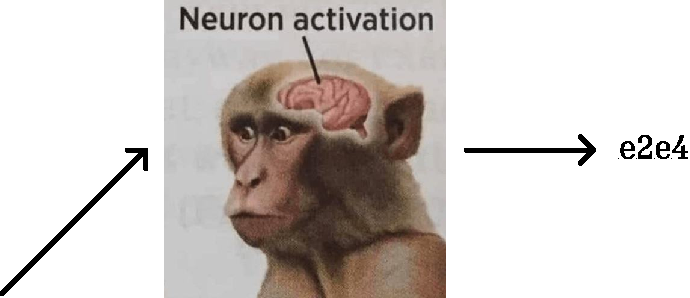
\includegraphics[width=0.8\linewidth]{../assets/slides/human.pdf}}}

            \visible<3->{\subfloat{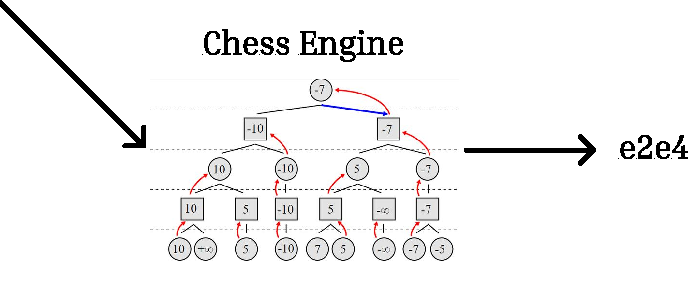
\includegraphics[width=0.8\linewidth]{../assets/slides/computer.pdf}}}
        \end{figure}
    \end{column}
\end{columns}
\end{frame}

\begin{frame}
\frametitle{Ajedrez como árbol}
\begin{figure}
    \centering
    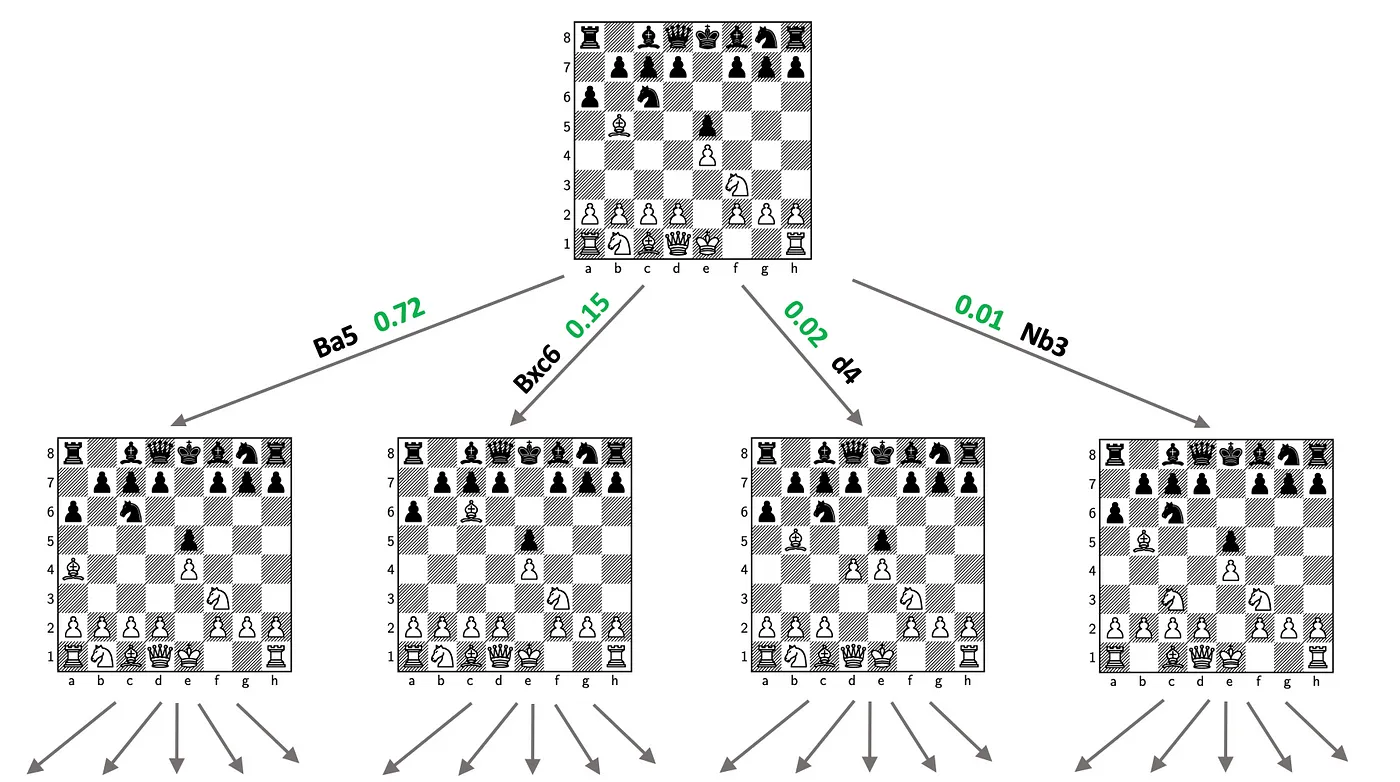
\includegraphics[width=1.0\linewidth]{../assets/slides/chess_tree.png}
\end{figure}
\end{frame}

\begin{frame}
\frametitle{Motores de ajedrez (Chess Engines)}
\begin{columns}
    \begin{column}{0.5\textwidth}
        \begin{itemize}
            \item<1-> Exploran el árbol de juego (Minimax, MCTS, etc.)
            \item<2-> Utilizan funciones de evaluación en las hojas
            \item<3-> La evaluación se propaga hacia arriba, según el algoritmo
        \end{itemize}
    \end{column}
    \begin{column}{0.6\textwidth}
        \begin{figure}
            \centering
            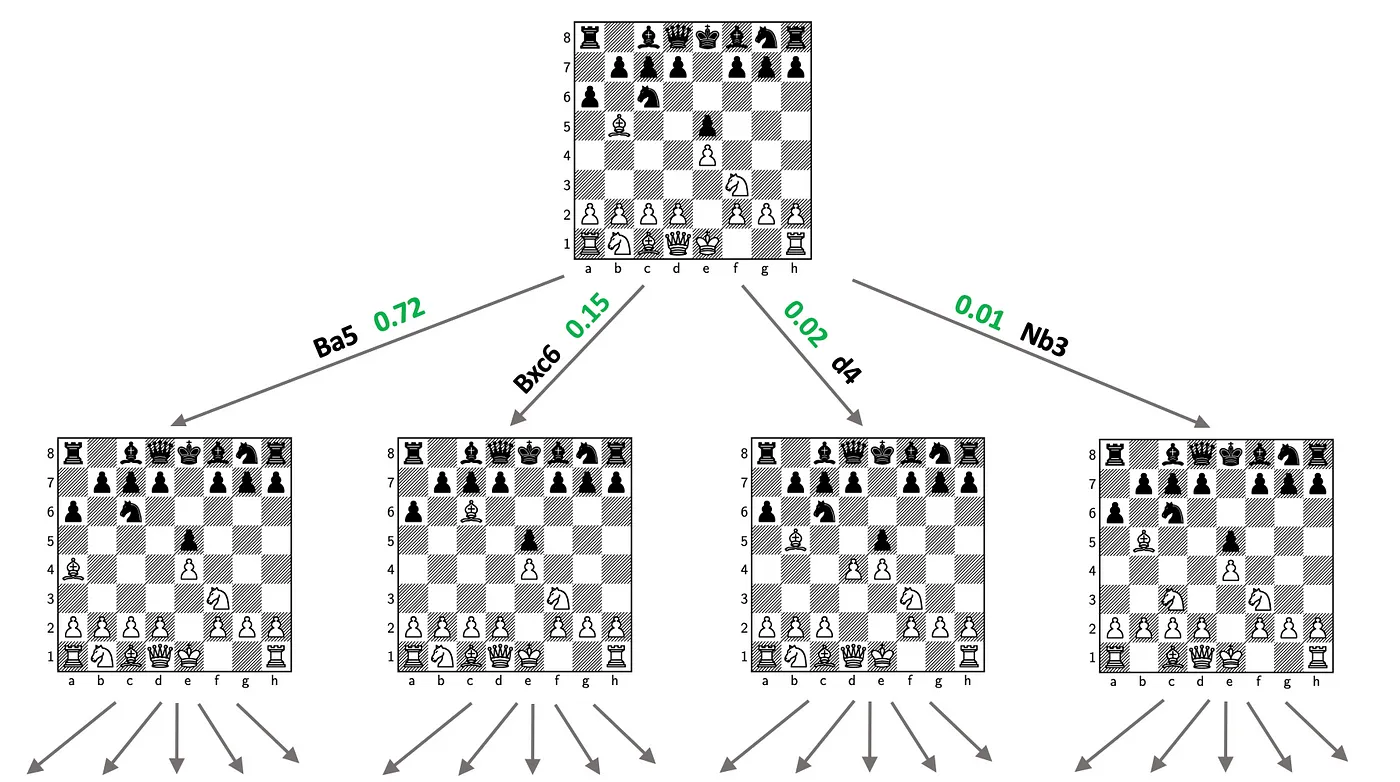
\includegraphics[width=0.9\linewidth]{../assets/slides/chess_tree.png}
        \end{figure}
    \end{column}
\end{columns}
\end{frame}

\begin{frame}
\frametitle{Función de evaluación o \enquote{eval}}
\begin{figure}
    \centering
    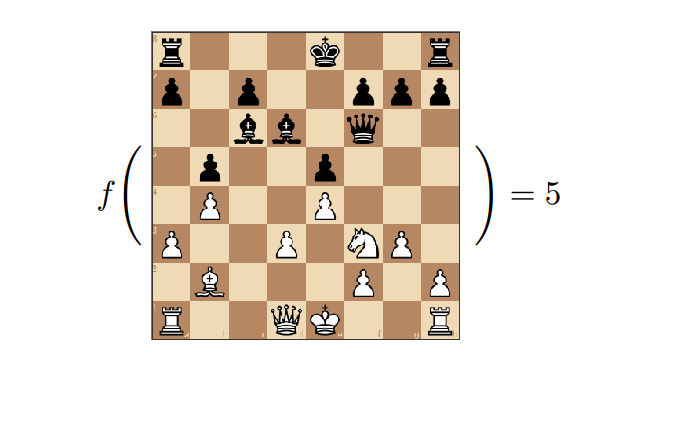
\includegraphics[width=0.8\linewidth]{../assets/slides/eval.png}
\end{figure}
\begin{center}
Intentan resumir todo el subárbol en un solo número. \\
En general son creadas \textit{artesanalmente}
\end{center}
\end{frame}

\begin{frame}
\frametitle{(adelanto) Feature sets: ¿Cómo transformar la posición a un vector para usar NNs?}
\begin{figure}
\centering
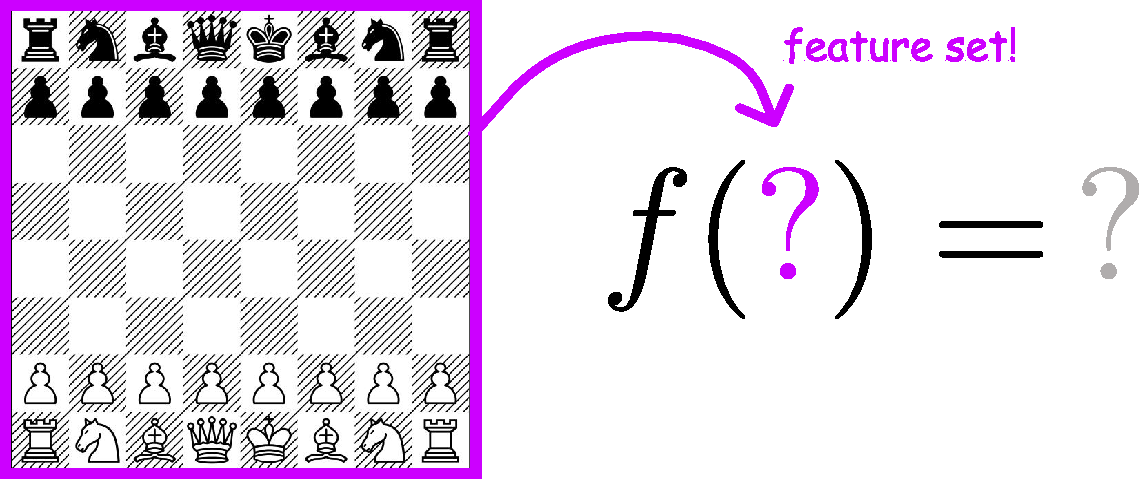
\includegraphics[width=1.0\linewidth]{../assets/slides/fs_motiv2.pdf}
\end{figure}
\end{frame}

\begin{frame}
\frametitle{Motores de ajedrez (breve historia)}
\begin{itemize}
    \item<1-> \textbf{1950s}: Se desarrollan los primeros \textit{algoritmos} de ajedrez
    \item<2-> \textbf{1960s+}: Aparecen los primeros \textit{motores de ajedrez}, lentos y débiles
    \item<3-> \textbf{1997} (hito): IBM DeepMind vence a Garry Kasparov en un torneo (superhuman)
    \item<4-> \textbf{2017 y 2018}: Google DeepMind publica AlphaGo Zero y su sucesor AlphaZero
    \begin{itemize}
        \item se reemplaza la función de evaluación por una red neuronal
    \end{itemize}
    \item<5-> \textbf{2018}: Yu Nasu introduce las redes \reflectbox{NNUE} para Shogi
    \item<6-> \textbf{2020}: Stockfish 12 introduce redes \reflectbox{NNUE} en su evaluación
    \begin{itemize}
        \item se utilizan a la par de evaluaciones artesanales
    \end{itemize}
    \item<7-> \textbf{2024}: Stockfish 16.1 elimina todo aspecto humano de su evaluación, todo es mediante redes neuronales
\end{itemize}
\end{frame}

\begin{frame}
\frametitle{Plan de la tesis}
El objetivo principal es \textbf{proponer y evaluar novedosos feature sets}. \pause Además, \textbf{probar una técnica de entrenamiento} no convencional. \\
\pause
\vspace{1em}
El plan de la presentación es el siguiente:
\begin{itemize}
\item<3-> Implementación de un motor de ajedrez clásico
\item<4-> Definición y ejemplos de feature sets
\item<5-> Introducción a las redes \reflectbox{NNUE}
\item<6-> Entrenamiento de las redes \reflectbox{NNUE}
\item<7-> Experimentos
\end{itemize}
\end{frame}

% \begin{frame}{Contenido}
% \tableofcontents
% \end{frame}

\section{Engine implementation}

Building chess engines is a very discussed topic in the history of chess and thus very well documented. The Chess Programming Wiki (CPW) \cite{cpw} is the best source of information to reference, which I will base my engine on. I aim to build a single-threaded classic engine and only make use of the most prominent optimizations to keep it simple. The engine strength is not that relevant, as it is only a tool to measure the relative performance of board encodings. However, a competent one is required.

Note that implementing the engine is not the main focus of this work, so some simplifications have been made to this chapter to keep it brief and simple. \\

Classic chess engines are composed of two main components: \textbf{the search} and \textbf{the evaluation}. The search is the process of exploring the tree of possible moves, which is what this chapter is about. The evaluation determines how good the positions are for who plays. As I mentioned in the introduction, classic engines used to use hand-crafted evaluations based on human knowledge. In my case, I will replace it entirely with a neural network, explained in the following chapters.

\subsection{Minimax search}

A position $p$ in chess is the state of the board with any other relevant information, like castling rights and the 50-move clock. Given a position $p$, we can call $f(p)$ its evaluation, a number that provides an assessment of how good the position is, computed either by a hand-crafted function or a neural network.

One approach to determinate the best move could be to evaluate all possible positions that can be reached with a single move and choose the one that leads to the highest evaluation for the player who made the move. This idea can be extended to consider actions taken by the other player, and so on, to a fixed depth. Formally, this is called the minimax search algorithm \cite{minimax-survey:1995}.

In a minimax tree search there are two kinds of nodes: maximizing nodes and minimizing nodes. 

\begin{itemize}
\item \textbf{Maximizing nodes} are the ones where the player to move is our player. These nodes want to put the player in the best possible position, so they choose the action that maximizes the evaluation. Note that the root node is a maximizing node.
\item \textbf{Minimizing nodes} are the ones where the player to move is the opponent. These nodes want to put the player in the worst possible position, so they choose the action that minimizes the evaluation.
\end{itemize}

The algorithm recursively explores the tree to a fixed depth, evaluating the positions at the leaves with $f$. The evaluation is then propagated up the tree, alternating between maximizing and minimizing nodes, until it reaches the root node. The best move is the one that leads to the highest evaluation at the root node.

Usually we don't want to run the search to a fixed depth, but rather for a fixed amount of time. The algorithm itself runs to a fixed depth so iterative deepening is implemented. Iterative deepening runs the search in a loop, staring from depth 1 and increasing it by one each iteration until the time runs out. This way the best move found so far is always available. Note that we can't draw conclusions from any unfinished search, so the best move is the one found at the last iteration. This approach, when combined with a transposition table (a cache for evaluations) is very effective, making next iterations faster. \\

The actual implementation I did was a variation of the minimax algorithm called negamax. Negamax is a simplification of minimax that takes advantage of the zero-sum property of chess, meaning that an evaluation for a player is equivalent to the negation of the evaluation in the opponent's point of view. Instead of having two kinds of nodes, all nodes are maximizing nodes and the evaluation is negated after the recursion. This simplifies the implementation.

\subsection{Quiescence search}

The search algorithm runs to a fixed depth, which causes a horizon effect. The horizon effect manifests when the search stops at a position where a negative event (such a capture) is inevitable but due the fixed depth, the search results in weaker moves in an effort to avoid the inevitable (prefers branches where the capture has not happened yet).

To fix this, instead of returning the evaluation of the position at the leaves, an additional smaller search is done which only considers captures. This way the search can continue until a \enquote{quiet} position is reached, where no captures are available.

Since most of the positions the network will be evaluating are quiet due the quiescence search, it is important to make sure that the training set reflect that. Later on, only positions that are quiet will be used to train the network.

\subsection{Optimizations}

Many optimizations were made to the engine to make it reach a decent depth in a reasonable time, which makes the engine stronger. There are no novel improvements, most are well-known techniques that have been used in engines for decades and can be found in the Chess Programming Wiki \cite{cpw}.

The most prominent optimizations implemented are:

\begin{itemize}
\item \textbf{Alpha-beta pruning}: a way to eliminate big portions of the search tree by using the branch-and-bound technique. It allows to prune branches that are guaranteed to be worse than the best move found so far. This means that it doesn't affect the result of the search, it only makes it faster.

Each node in the search tree has two values associated with it: $\alpha$ and $\beta$. $\alpha$ is the best value found so far that the maximizing player can guarantee up to that node. $\beta$ is the best value found so far that the minimizing player can guarantee up to that node. Note that $\alpha \le \beta$ and the maximizing player tries to \enquote{push} $\alpha$ up and the minimizing player tries to \enquote{pull} $\beta$ down.

When a node is visited, the algorithm checks if $\alpha \ge \beta$. If this is the case, the branch can be pruned because the minimizing player can guarantee a value of $\beta$, which is worse than the best value found so far.

\item \textbf{Move ordering}: the order in which the moves are evaluated can have a big impact on the effectiveness of the alpha-beta pruning. There are a couple of ways to improve move ordering, the most important being:
\begin{itemize}
\item \textbf{MVV/LVA} The most valuable victim, least valuable attacker is a simple heuristic that orders the moves by the value of the captured piece minus the value of the attacking piece. This way the most valuable captures are evaluated first, which are more likely to cause a cutoff.
\end{itemize}

\item \textbf{Transposition table}: During search, a position may be visited many times with different sequences of moves. This is called a transposition. The transposition table is a large hash table storing information about positions that have already been visited. This way, if a position is visited again, the engine can use the stored information to avoid re-evaluating it.

Even if the depth of the stored evaluation is lower than the current depth (insufficient to draw conclusions at the current depth), it can still be used to improve the move ordering.

\end{itemize}

Many other optimizations were made and can be found in the documented code.

%- principal variation (mainline)
%- null move prunning
%- late move reductions
%- history moves, killer moves

\subsection{Implementation details}

%- Rust
%- I/O with UCI protocol
%- move generation using a fast library
%- POSITION STACK
%- time control

The engine is implemented in the Rust programming language. It uses the standard UCI protocol to communicate via standard input/output.

The most performance critical part of the engine aside from the evaluation is move generation, that is, given a position, list all available moves and make them.
Fortunately there is a battle-tested library for it called \textit{shakmaty}. The library provides a copy-make interface instead of a make-unmake one, so I have to rely on a stack of positions when doing recursion.

Time control is hard-coded to use the increment plus 2\% of the remaining time per move. Experiments run at a fixed time per move, so this is used in the Lichess arena.

By default the engine uses 128 MB of memory for the transposition table. This value will be used throughout the experiments and in the arena.


\newcommand{\white}{\fullmoon}
\newcommand{\black}{\newmoon}

\newcommand{\bigtimes}{\mathop{\raisebox{-0.5ex}{\scalebox{2}{$\times$}}}}

% https://texdoc.org/serve/chessboard/0
\newcounter{pieceindex}
\newcommand{\pieceBoard}{
    \newcount\pieceindex
    \setcounter{pieceindex}{0}
    \raisebox{-7ex}{
        \centering
        \chessboard[
            tinyboard,
            showmover=false,
            margin=false,
            padding=false,
            hlabel=false,
            vlabel=false,
            pgfstyle={text},
            %text=\fontsize{1.2ex}{1.2ex}\bfseries\sffamily \thepieceindex \stepcounter{pieceindex}, %  \currentwq
            text=\fontsize{1.2ex}{1.2ex}\bfseries\sffamily \currentwq,
            markboard
        ]
    }
}
\newcommand{\pieceRolesTable}{
    \begin{tabular}{|l|}
        \hline
        \sympawn\ Pawn \\
        \hline
        \symknight\ Knight \\
        \hline
        \symbishop\ Bishop \\
        \hline
        \symrook\ Rook \\
        \hline
        \symqueen\ Queen \\
        \hline
        \symking\ King \\
        \hline
    \end{tabular}
}
\newcommand{\pieceColorsTable}{
    \begin{tabular}{|l|}
        \hline
        $\white$ White \\
        \hline
        $\black$ Black \\
        \hline
    \end{tabular}
}

\newcommand{\featureset}[1]{\textsc{#1}}
\newcommand{\feature}[1]{$\langle$#1$\rangle$}


\section{Feature sets (board encodings)}

To evaluate chess positions, the engine will use a neural network with an architecture explained in detail in the next chapter. In this chapter, I will show how to build the one-dimensional input vector for such network, which can be described entirely by a feature set. \\

A feature set is a set with a predicate attached to it. The elements can be anything, but usually we want to represent chess concepts like piece locations, piece roles, colors, etc. We may want to represent more complex patterns, so we can build feature sets by taking the cartesian product of smaller sets. The predicate $\bm{P(e)}$ defines if the element or pattern $e$ is present (or \textit{active}) in the (implicit) position. The predicate is generally written using natural language.

Formally, given a set of concepts or tuples $\bm{S}$ and a predicate $\bm{P}$, we can define a feature set as ${\bm S}_{\bm P}$, where each element is called a feature. Each feature corresponds to a value in a vector, which will be set to $1$ if the predicate is satisfied for that element in the position, and $0$ otherwise. This is the vector that will be used as input to the neural network. \\

Let's consider some basic sets of concepts. For example, the following sets describe positional information about the board:

\begin{center}
\begin{tabular}{cc}

$\begin{aligned}[t]
\featureset{Files} &= \{a, b, ..., h\} \\
\featureset{Ranks} &= \{1, 2, ..., 8\} \\
\featureset{Squares} &= \{a1, a2, ..., h8\}
\end{aligned}$

&

\raisebox{-10ex}{
\chessboard[
    tinyboard,
    showmover=false,
    pgfstyle={text},
    %text=\fontsize{1.2ex}{1.2ex}\bfseries\sffamily \thepieceindex \stepcounter{pieceindex}, %  \currentwq
    text=\fontsize{1.2ex}{1.2ex}\bfseries\sffamily \currentwq,
    markboard
]
}

\end{tabular}
\end{center}

And the following describe information about the pieces:

\begin{center}
$\begin{aligned}[t]
\featureset{Roles} &= \text{\{
    \sympawn\ Pawn,
    \symknight\ Knight,
    \symbishop\ Bishop,
    \symrook\ Rook,
    \symqueen\ Queen,
    \symking\ King\}}\textsuperscript{1} \\
\featureset{Colors} &= \text{\{\white\ White, \black\ Black\}}
\end{aligned}$
\end{center}

\footnotetext[1]{The color of the pieces have no meaning in the definition. They are present for illustrative purposes.}

For example, consider the feature set $(\featureset{Files} \times \featureset{Colors})_{P}$ where $P$ is defined like $P(\langle f, c \rangle): $ there is a piece in file $f$ with color $c$. A feature in this set will be active if there is at least one piece in the board that makes the predicate true. In this case, disregarding any other kind of information, like the piece's role.
Another possible feature set could be $(\featureset{Files} \times \featureset{Roles})_{Q}$, with a similar interpretation. An illustration of the active features of these two feature sets is shown in Figure \ref{fig:active_features}.

Note that $\featureset{Squares}_R$ is equivalent to $(\featureset{Files} \times \featureset{Ranks})_R$ $\forall R$.

\begin{figure}[H]
\centering

\begin{tabular}{cc}
\raisebox{-7ex}{
\chessboard[
    tinyboard,
    showmover=false,
    hlabel=false,
    setwhite={kc3, nc2, pa2, Pd4},
    addblack={Kc8,bh7, pa7}
]
}

&

\begin{tabular}{|c|p{4cm}|p{4cm}|p{0cm}}
\cline{2-3}
\multicolumn{1}{c|}{} & \multicolumn{2}{c|}{\centering Feature set} \\
\cline{2-3}
\multicolumn{1}{c|}{} & \centering $(\featureset{Files} \times \featureset{Colors})_{P}$ & \centering $(\featureset{Files} \times \featureset{Roles})_{Q}$ & \\
\cline{1-3}
Active features &
\feature{a, \white}, \feature{a, \black}, \feature{c, \black}, \feature{c, \white}, \feature{d, \white}, \feature{h, \black} &
\feature{a, \sympawn}, \feature{c, \symking}, \feature{c, \symknight}, \feature{d, \sympawn}, \feature{h, \symbishop} \\
\cline{1-3}

\multicolumn{3}{c}{
\makecell{
~\\
$P(\langle f,c \rangle)$: there is a piece in file $f$ with color $c$.\\
$Q(\langle f,r \rangle)$: there is a piece in file $f$ with role $r$.
}    
}

\end{tabular}
\end{tabular}

\caption{Active features of two feature sets for the same board.}
\label{fig:active_features}
\end{figure}

\subsection{Sum $\oplus$}

% what to talk about:
% we want the network to find patterns between the two sets
% some feature sets can be built merging the features of two or more sets

The sum (or concatenation) of two feature sets $\featureset{A}$ and $\featureset{B}$, denoted by $\featureset{A} \oplus \featureset{B}$, is a new feature set comprised of the features of both sets. These features do not interfere with each other at all. Formally, given two feature set $S_P$ and $T_Q$, we can define the sum operator as
\begin{equation*}
S_P \oplus T_Q = {(S \cup T)}_R
\end{equation*}
\begin{equation*}
    \text{where } R(e) = \begin{cases}
        P(e) & \text{if } e \in S \\
        Q(e) & \text{if } e \in T
    \end{cases}
\end{equation*}

The sum operator is useful when we want to let the network find patterns combining information between two sets of features.

Even though the two operands are feature sets, they are usually called \enquote{feature blocks} since they are part of a larger feature set. The final feature set that is used for training is a sum of many feature blocks.

\subsection{Product $\times$}

The product of two feature sets $\featureset{A}$ and $\featureset{B}$, denoted by $\featureset{A} \times \featureset{B}$, is a new feature set where each new feature is a combination of the features of both sets. One way to interpret this is that each new feature will be active if both features in the original sets are active \textit{at the same time}. Formally, given two feature sets $S_P$ and $T_Q$, we can define the product operator as
\begin{equation*}
S_P \times T_Q = {(S \times T)}_{R}
\end{equation*}
\begin{equation*}
\text{where } R(\langle e_0, e_1 \rangle) = P(e_0)\ \land\ Q(e_1)
\end{equation*}

This operation is not that useful because it requires both predicates to be independent from each other. This will be used specifically to define the \featureset{King-All} feature set and potentially its variations.

\newpage
\subsection{Known feature sets}

In this section, I will define two of the most important feature sets known and used extensively in existing engines.

\subsubsection{\mdseries\featureset{All}}

This feature set is the most natural encoding for a chess position. It is called \enquote{All} because it captures all the pieces. There is a one-to-one mapping between pieces in the board and features:

\begin{center}
    $\featureset{All}:\ (\featureset{Squares} \times \featureset{Roles} \times \featureset{Colors})_{P}$ \\
    $P(\langle s, r, c \rangle)$: there is a piece in square $s$ with role $r$ and color $c$\\
\end{center}

Tuples in this set are \textit{active} if there is a piece in the board that matches the role, color and position of the tuple. For example, the tuple \feature{e4, \sympawn, \white} is active if there is a white pawn in the square e4. This way, for every possible piece, in every possible position, there is a feature. The set has $64*6*2=$\textbf{ 768 features}, which makes it very small and it is very easy to compute which features are active.

\subsubsection{\mdseries\featureset{King-All}}

Another feature set built on top of $\featureset{All}$ is the \featureset{King-All} feature set, or \enquote{KA} for short. For every possible position where the king of the side to move can be, there is a complete copy of the \featureset{All} set:

\begin{center}
    $\featureset{King-All} = \featureset{Square}_{K} \times \featureset{All}$ \\
    $K(s)$: $s$ is the square of the king of the side to move\\
\end{center}

This encoding allows the network to understand better the position of the pieces in relation to the king, which is very tied to the evaluation of the position.

The number of features is $64*768=$ \textbf{49152 features}. There is a variation of this feature set called \enquote{KP} which is the same but it does not consider the enemy king, reducing the amount of features to 40960. There are other variations, such as \featureset{KAv2} or notably \featureset{KAv2\_hm} that is currently the latest feature set used by Stockfish 16.1.

The features in this set are easy to compute like in $\featureset{All}$, but since the number of features is much larger, it is a lot harder to train and use in practice. I will restrain this work to smaller feature sets that are easier to manage.

\newpage
\subsection{Indexing}

% The input to the network is a one-dimensional vector, so we need a way to map the tuples (elements are trivial) in a feature set to elements in the input vector. The correct index for a tuple is computed using the order of the sets in the cartesian product and the size of each set, like strides in a multi-dimensional array. For this to work, each element in a set $S$ must correspond to a number between $0$ and $|S| - 1$. For example, the feature set $A \times B \times C$ has $|A| \times |B| \times |C|$ elements, and the tuple $(a, b, c)$ is mapped to the element indexed at $a \times |B| \times |C| + b \times |C| + c$. The same striding logic applies to feature sets built with the sum operator, recursively.

We need a way to map the tuples in a feature set to elements in the input vector. The correct index for a tuple is computed using the order of the sets in the cartesian product and the size of each set, like strides in a multi-dimensional array. For this to work, each element $e$ in a set $S$ must correspond to a number between $0$ and $|S| - 1$, we call this bijective mapping $I(e)$.

For example, the feature set $(A \times B \times C)_{P}$ has $|A| \times |B| \times |C|$ features, and the feature \feature{a, b, c} is mapped to the element indexed at $I(a) \times |B| \times |C| + I(b) \times |C| + I(c)$. The same striding logic applies to feature sets built with the sum and product operators, recursively.

\subsection{Dead features}

Consider the $\featureset{All}$ feature set. For every position, role and color each piece could be, there is a feature. There are 16 tuples in the set that will never be active: \feature{a8..h8, \sympawn, \white} and \feature{a1..h1, \sympawn, \black} that correspond to the white pawns in the last rank and the black pawns in the first rank. This is because pawns promote to another piece when they reach the opponent side of the board, so no pawns will ever be found there. Effectively, these will be dead neurons in the network, but this way we can keep the indexing straightforward. Most feature sets will have dead features, and the same logic applies.

\subsection{Summary}

\begin{enumerate}
\item $\bm S$: set of concepts (roles, colors, squares, files, ranks, etc.).
\item $\bm{P(e)}$: predicate that defines when the feature $e$ is present in the (implicit) position.
\item ${\bm S}_{\bm P}$: a feature set. Every element in $S$ is a feature. Features in $S$ that satisfy $P$ are \textit{active}.
\item $S_P \times T_Q={(S \times T)}_{R}$ where $R(\langle e_0, e_1 \rangle) = P(e_0)\ \land\ Q(e_1)$
\item $S_P \oplus T_Q={(S \cup T)}_R$ where $R(e) = \begin{cases}
        P(e) & \text{if } e \in S \\
        Q(e) & \text{if } e \in T
    \end{cases}
$

\end{enumerate}

\section{Efficiently updatable neural networks}

NNUE (\reflectbox{NNUE} Efficiently updatable neural network) is a neural network architecture that allows for very fast subsequent evaluations when changes in the input are minimal. It was invented for Shogi by Yu Nasu in 2018 \cite{nnue:2018}, later adapted to Chess for use in Stockfish in 2019. Most of the information described in this chapter can be found in the excellent Stockfish NNUE documentation \cite{nnue-pytorch}. \\

NNUE operates on the following principles:

\begin{itemize}
    \item \textbf{Input sparsity}: The network should have a relatively low amount of non-zero inputs, determined by the chosen feature set. The presented feature sets have between 0.1\% and 2\% of non-zero inputs for a typical position. Having a low amount of non-zero inputs places a low upper bound on the time required to evaluate the network in its entirety, which can happen using some feature sets like \featureset{King-All} that triggers a complete refresh when the king is moved.
    \item \textbf{Efficient updates}: From one evaluation to the next, the number of inputs changes should be as low as possible. This allows for the most expensive part of the network to be efficiently updated, instead of recomputed from scratch.
    \item \textbf{Simple architecture}: The network should be composed of a few and simple operators, that can be efficiently implemented with low-precision arithmetic in integer domain using CPU hardware (quantization).

\end{itemize}

There is a tradeoff between inference time and quality of the predictions, which affect the amount of nodes evaluated. If the inference is faster, more nodes can be evaluated thus reaching deeper in the search tree. Having higher quality predictions, which usually comes with a more complex model and/or feature set, can make stronger moves with shallower searches, and may improve prunning.

Models must be so much better to compensate the slowdown in inference when using bigger models or more complex feature sets. This is a tradeoff that will appear further in the experiments.

\subsection{Layers}

For this thesis, I have chosen to use a very simple NNUE architecture, which consist of two linear (fully connected) layers and clipped ReLU activations. In the literature, there are other architectures that make use of polling layers, sigmoid activations and others. Since this work is about experimenting with feature sets, I have chosen to stick with something simple that has been proven to achieve good results.

\paragraph[short]{Linear layer} A linear layer is a matrix multiplication followed by a bias addition. It takes \textbf{in\_features} input values and produces \textbf{out\_features} output values. The operation is $\bm{y} = \bm{W} \bm{x} + \bm{b}$, where:

\begin{enumerate}
\item $\bm{x}$ the input column vector of shape \textbf{in\_features}.
\item $\bm{W}$ the weight matrix of shape (\textbf{out\_features}, \textbf{in\_features}).
\item $\bm{b}$ the bias column vector of shape \textbf{out\_features}.
\item $\bm{y}$ the output column vector of shape \textbf{out\_features}.
\end{enumerate}

If we call $\bm{A_i}$ the $i$-th column of the weight matrix $\bm{W}$, the operation $\bm{W} \bm{x}$ can be simplified to \enquote{if $\bm{x_i}$ is not zero, take the column $\bm{A_i}$, multiply it by $\bm{x_i}$ and add it to the result}. This means that we can skip the processing of columns that have a zero input, as depicted in Figure \ref{fig:linear_comparison}.

\begin{figure}[H]
\centering
\subfloat[\centering Linear layer]{{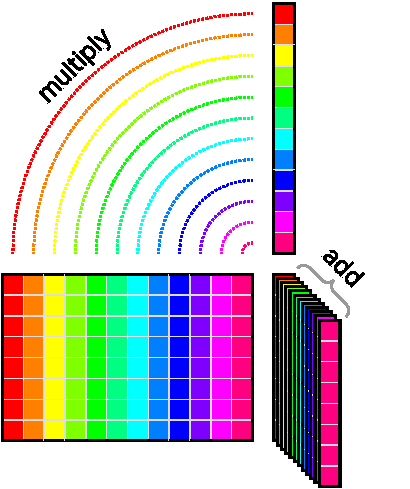
\includegraphics[width=5cm]{../assets/nnue/mv.pdf} }}%
\qquad
\subfloat[\centering Linear layer with sparse inputs]{{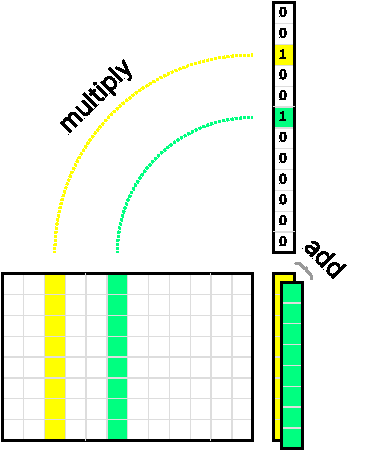
\includegraphics[width=5cm]{../assets/nnue/mvs.pdf} }}%
\caption{Linear layer operation comparison. Figures from \cite{nnue-pytorch}.}
\label{fig:linear_comparison}
\end{figure}

In the case of the first layer, the input is a very sparse one-hot encoded vector. This means that very few columns will have to be processed and the multiplication can be skipped altogether, due all inputs being either 0 or 1. Skipping the multiplication reduces the operations to only additions and subtractions.

\paragraph[short]{Clipped ReLU} This is a simple activation that clips the output in the range $[0, 1]$. The operation is $\bm{y=\min(\max(x,0),1)}$.
The output of this activation function is the input for the next layer, and because of the aggresive \textit{quantization} that will be described later, it is necessary to restrain the values so it does not overflow. \\

\subsection{Efficient updates}

When running a depth-first search algorithm, the state of the position is updated every time the algorithm \textit{makes} and \textit{unmakes} moves, usually before and after the recursion.
NNUEs are designed to work with this kind of search, since every time the algorithm \textit{makes} (or \textit{unmakes}) a move, the changes in the position are minimal (at most two pieces are affected in \featureset{All}), meaning that the amount of features becoming active or inactive is minimal as well. This is depicted in Figure \ref{fig:updates_tree}.

\begin{figure}[H]
\centering
\storechessboardstyle{3x3}{tinyboard,maxfield=c3,margin=false,showmover=false,hlabel=true,vlabel=true,pgfstyle=color,color=blue}
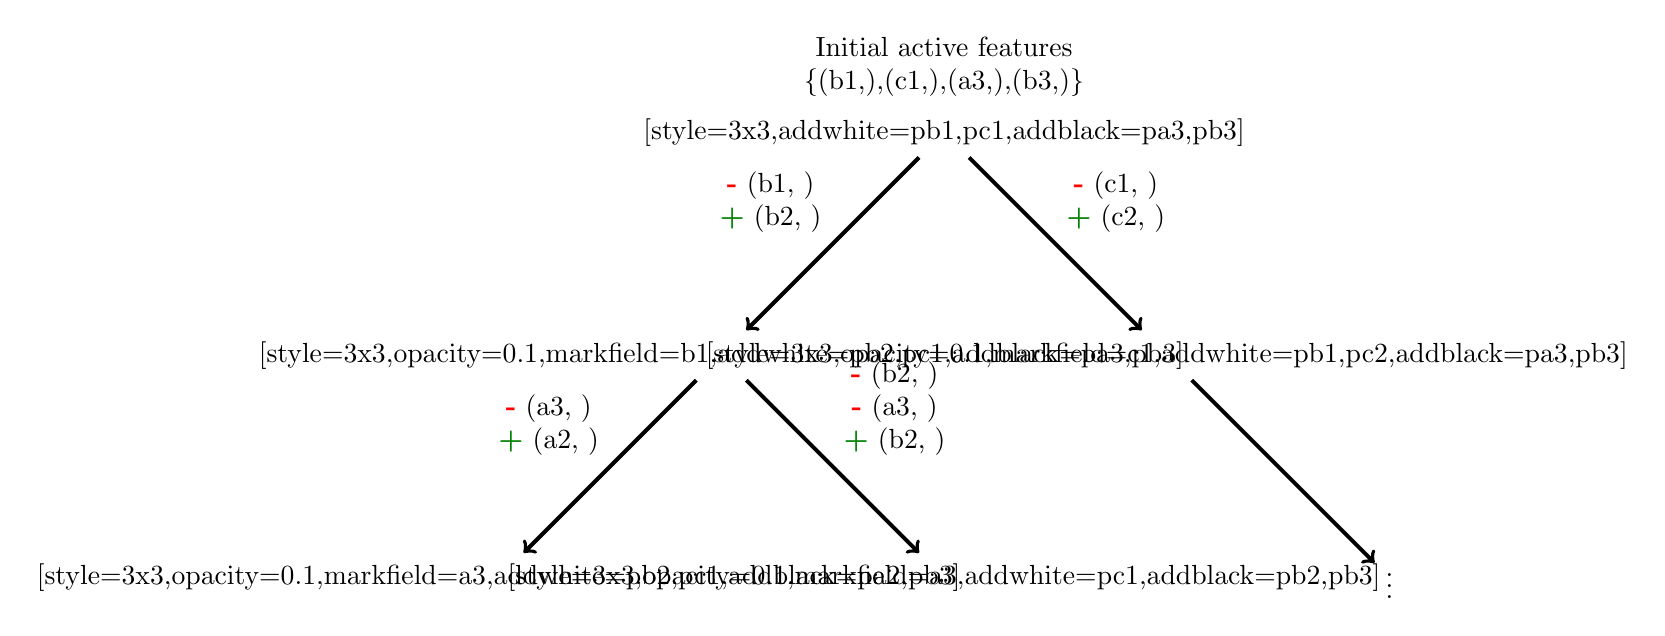
\begin{tikzpicture}[
    node distance=4cm,
    line width=0.5mm,
    auto
]

    \node[label={[align=center]Initial active features \\ \{(b1,\white),(c1,\white),(a3,\black),(b3,\black)\}}] (A) {\chessboard[style=3x3,addwhite={pb1,pc1},addblack={pa3,pb3}]};

    % childs of A
    \node (B) [below left of=A] {\chessboard[style=3x3,opacity=0.1,markfield={b1},addwhite={pb2,pc1},addblack={pa3,pb3}]};
    \node (C) [below right of=A] {\chessboard[style=3x3,opacity=0.1,markfield={c1},addwhite={pb1,pc2},addblack={pa3,pb3}]};

    % childs of B
    \node (D) [below left of=B] {\chessboard[style=3x3,opacity=0.1,markfield={a3},addwhite={pb2,pc1},addblack={pa2,pb3}]};
    \node (E) [below right of=B] {\chessboard[style=3x3,opacity=0.1,markfield={a3},addwhite={pc1},addblack={pb2,pb3}]};

    % childs of C
    \node (F) [below right of=C] {\vdots};

    % arrows of A
    \path[<-] (B) edge node[align=center] {\textbf{{\color{Red}-}} (b1, \white) \\ \textbf{{\color{Green}+}} (b2, \white)} (A);
    \path[->] (A) edge node[align=center] {\textbf{{\color{Red}-}} (c1, \white) \\ \textbf{{\color{Green}+}} (c2, \white)} (C);
    
    % arrows of B
    \path[<-] (D) edge node[align=center] {\textbf{{\color{Red}-}} (a3, \black) \\ \textbf{{\color{Green}+}} (a2, \black)} (B);
    \path[->] (B) edge node[align=center] {\textbf{{\color{Red}-}} (b2, \white) \\ \textbf{{\color{Red}-}} (a3, \black) \\ \textbf{{\color{Green}+}} (b2, \black)} (E);

    % arrows of C
    \path[<-] (F) edge node[align=center] {} (C);

\end{tikzpicture}
\caption{Partial tree of feature updates (\textcolor{Red}{removals} and \textcolor{Green}{additions}) for $(\featureset{Squares} \times \featureset{Colors})$ (white's point of view) in a simplified 3x3 pawn-only board.}
\label{fig:updates_tree}
\end{figure}

To take advantage of this during search, instead of computing all the features active in a position and then evaluate the network in its entirety, we can \textbf{accumulate} the output of the first linear layer and update it with when the position changes. Linear layers can be computed adding the corresponding columns of the weight matrix into the output, so when a feature becomes active or inactive, we can add or subtract the corresponding column to the output. When the evaluation is needed, only the next layers (usually small) have to be computed. \\

Recall that the way I defined feature sets, they always encode the position from one white's point of view. This means that its not possible to use the same \textbf{accumulator} for both players. So when running the search, we have to keep two accumulators, one for white and one for black, where the black board is flipped and has the colors swapped to match the point of view.

% [agregar grafico de black → white board → encode, para mostrar como se flipea / swapea. arriba el white → encode; poner los features activos quizas?]

%\begin{figure}[h]
%\centering
%
%\begin{tabular}{ccccc}
%
%\raisebox{-7ex}{\chessboard[
%    setfen=2Qb4/5pk1/p5p1/1pp3Pp/3qPp1P/P7/1PP1B3/1K6 w - - 1 29,
%    tinyboard,
%]}
%
%&
%
%&
%
%
%&
%
%$\xrightarrow{\text{encode}}$
%
%&
%
%Features
%
%\\
%
%\raisebox{-7ex}{\chessboard[
%    setfen=2Qb4/5pk1/p5p1/1pp3Pp/3qPp1P/P7/1PP1B3/1K6 b - - 1 29,
%    tinyboard,
%]}
%
%&
%
%$\xrightarrow{\text{flip vertically}}$
%
%&
%
%\raisebox{-7ex}{\chessboard[
%    setfen=2Qb4/5pk1/p5p1/1pp3Pp/3qPp1P/P7/1PP1B3/1K6 b - - 1 29,
%    tinyboard,
%]}
%
%&
%
%$\xrightarrow{\text{swap colors}}$
%
%&
%
%\raisebox{-7ex}{\chessboard[
%    setfen=2qB4/5PK1/P5P1/1PP3pP/3QpP1p/p7/1pp1b3/1k6 w - - 1 29,
%    tinyboard,
%]}
%
%
%\end{tabular}
%\end{figure}


During search, the first layer is replaced by two accumualtors to take advantage of this. Figure \ref{fig:incr_update} depicts how the output of both accumulators is concatenated depending on which player is moving, to later be passed through the rest of the network which is computed as usual. 

\begin{figure}[H]
\centering
\makebox[\textwidth]{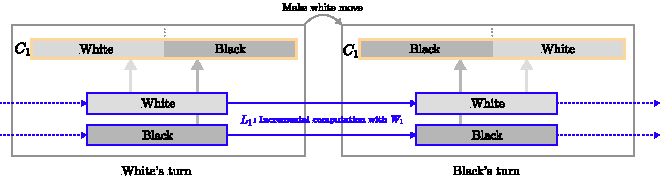
\includegraphics[width=\textwidth]{../assets/nnue/incremental_update.pdf}}
\caption{Concatenation of the first layer's output after a move is made. Inspired in a CPW figure.}
\label{fig:incr_update}
\end{figure}

\subsection{Network}

The network will be composed of three linear layers $L_1$ through $L_3$, each but the last one followed by a clipped ReLU activation $C_1$ and $C_2$. The network has two inputs: it takes the encoding (feature set) of a position from each player's point of view. Each encoding is passed through the same $L_1$ layer (same weights) and then the output is concatenated before passing it through the rest of the network. The first layer can be seen as a feature transformer, and it must share weights to allow for efficient updates. The network can be described as follows: \\

$\bm{N}$: number of features in the feature set

\begin{enumerate}
\itemsep-0.2em
\item $L_1 \times 2$: Linear from $\bm{N}$ to $\bm{M}$ ($\bm{W_1}$ weight, $\bm{b_1}$ bias)
\item $C_1$: Clipped ReLU of $\bm{2 * M}$
\itemsep0.2em
\item $L_2$: Linear from $\bm{2 * M}$ to $\bm{O}$ ($\bm{W_2}$ weight, $\bm{b_2}$ bias)
\itemsep-0.2em
\item $C_2$: Clipped ReLU of $\bm{O}$
\itemsep0.2em
\item $L_3$: Linear from $\bm{O}$ to $\bm{1}$ ($\bm{W_3}$ weight, $\bm{b_3}$ bias)
\end{enumerate}


The size of each layer is not fixed since it is a hyperparameter I will experiment with. The network architecture is depicted in Figure \ref{fig:network}, with example parameters.

\begin{figure}[H]
\centering
\makebox[\textwidth]{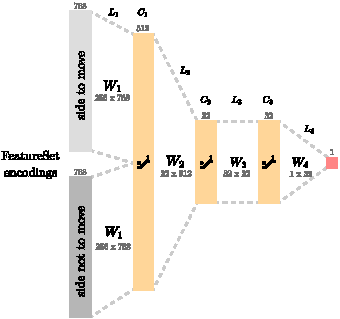
\includegraphics[width=10cm]{../assets/nnue/network.pdf}}
\caption{Neural network architecture with $\bm{N}=768$, $\bm{M}=256$, $\bm{O}=32$. Not to scale.}
\label{fig:network}
\end{figure}

\subsection{Quantization}

% https://github.com/official-stockfish/nnue-pytorch/blob/master/docs/nnue.md#quantization

Quantization is the process of converting the operations and parameters of a network to a lower precision. It is a step performed after all training has been done, which do happen in float domain. Floating point operations are too slow to achieve acceptable performance, as it sacrifices too much speed. This was necessary to implement to have a working engine.

Quantizing the network to integer domain will inevitable introduce some error, but it far outweights the performance gain. In general, the deeper the network, the more error is accumulated, but since NNUEs are very shallow by design, the error is negligible. At the end of the chapter I do an analysis of the error introduced by quantization.

Since the objective is to take advantage of modern CPUs that allow doing low-precision integer arithmetic in parallel with 8, 16, 32 or even 64 8-bit integer values at a time, we want to use the smallest integer type possible everywhere, to process more values at once.

\subsubsection{Stockfish quantization scheme}

\def\int#1{\texttt{int#1}}

In this thesis, I will use the same quantization scheme used in the engine Stockfish \cite{nnue-pytorch}, due its simplicity and it has been battle tested. It uses \int{8} $[-128, 127]$ for inputs and weights, and \int{16} $[-32768, 32767]$ where \int{8} does not fit the range of values we need.
To convert the float values to integer, we need to multiply the weights and biases by some constant to translate them to a different range of values. Each layer is different, so I'll go through each one.

%\begin{figure}[H]
%\centering
%\makebox[\textwidth]{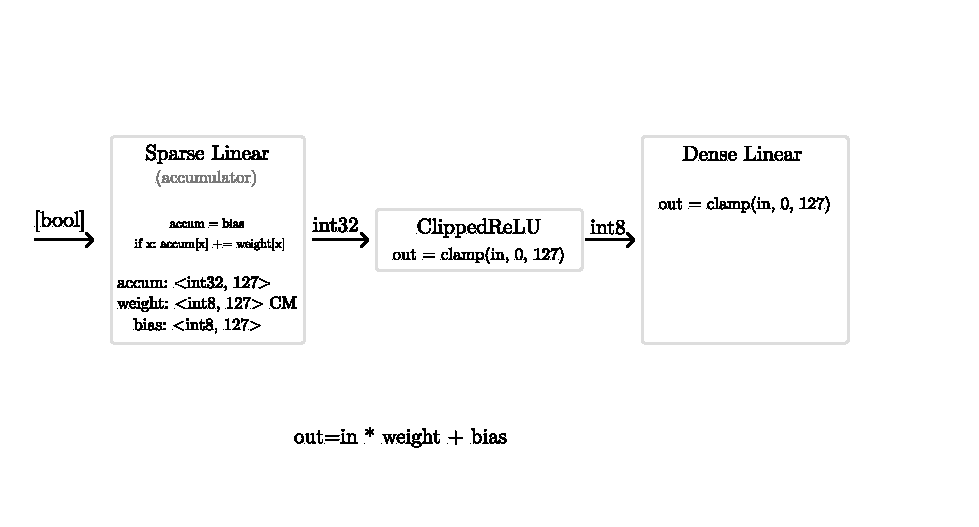
\includegraphics[width=\textwidth]{../%assets/nnue/quantization.pdf}}
%\caption{Simplified network showcasing all layers with %quantization values}
%\label{fig:quantization}
%\end{figure}

\paragraph[short]{Input} In float domain inputs are either $0.0$ or $1.0$, and since they are quantized to \int{8} we must scale them by $s_a=127$ (activation scale), so inputs are either $0$ or $127$. During inference, the input values are not computed since the first layer is an accumulator. However it is important to note that the rows being accumulated are scaled by $s_a=127$.

\paragraph[short]{ClippedReLU} The output of the activation in float domain is in the range $[0, 1]$ and we want to use \int{8} in the quantized version, so we can multiply by $s_a=127$ and clamp in the range [0, 127]. The input data type may change depending on the previous layer: if it comes from the accumulator, it will be \int{32}, and if it comes from a linear layer, it will be \int{16}.

% \paragraph[short]{Input} Since we are using accumualtors, there is not a real input to the model.
% Inputs are quantized to 8 bits, so the range of values is $-128..127$. Since the inputs are hot encoded, the float values are 0.0 or 1.0, so the quantized values are either 0 or 127.

\paragraph[short]{Accumulator (L1)}



The purpose of this layer is to accumulate rows of the first layer's weight matrix, which is stored in \int{16}. The values are stored in column-major order so a single row is contiguous in memory. Since we are accumulating potentially hundreds of values which are stored in \int{16} and scaled by $s_a=127$, we must accumulate in \int{32} to avoid overflows. The output of this layer will be the input for the ClippedReLU activation.

\paragraph[short]{Linear layer (L2 and L3)} The input to this layer will be scaled to the activation range because it takes the output of the previous ClippedReLU activation: $s_a \bm{x}$. We want the output to also be scaled to the activation range so it can be passed to the next: $s_a \bm{y}$.

To convert the weights to \int{8}, we must scale them by some factor $s_W=64$ (value used in Stockfish, efficient in SIMD because is just a shift): $s_W \bm{W}$. The value $s_W$ depends on how much precision we want to keep, but if it is too large the weights will be limited in magnitude. The range of the weights in floating point is then determined by $\pm \frac{s_a}{s_W}=\frac{127}{64}=1.984375$, and to make sure weights don't overflow, it is necessary to clip them to this range during training. The value $s_W$ also determinates the minimum representable weight step, which is $\frac{1}{s_W}=\frac{1}{64}=0.015625$.

The linear layer operation with the scaling factors applied looks like:

\begin{equation}
\begin{aligned}
s_a s_W \bm{y} &= (s_W \bm{W}) (s_a \bm{x}) + s_a s_W \bm{b} \\
\end{aligned}
\end{equation}
\begin{equation}
\begin{aligned}
s_a \bm{y} &= \frac{(s_W \bm{W}) (s_a \bm{x}) + s_a s_W \bm{b}}{s_W} \\
\end{aligned}
\end{equation}

From that equation we can extract that, to obtain the result we want, which is the output of the layer scaled to the activation range ($s_a \bm{y}$), we must divide the result of the operation by $s_W$ (2). Also that the bias must be scaled by $(s_a s_W)$. \\

The last linear layer (L3) is a bit different since there is no activation afterwards, so we don't want any scalings at all:

\begin{equation}
\begin{aligned}
\bm{y} = \frac{(s_W \bm{W}) (s_a \bm{x}) + s_a s_W \bm{b}}{s_a s_W}
\end{aligned}
\end{equation}

% no se tiene el mismo problema que en el accumulator layer porque la multiplicacion en SIMD se hace en 32 bits (osea sin hacer overflow), para despues aplicar clippedrelu a eso.

\subsection{Implementation}

The Stockfish repository provides an AVX2 implementation of the mathematical operations in C++. They have been carefully ported to Rust for this thesis. The implementation was thoroughly tested using the Pytorch model as reference (output match).

\subsubsection{Quantization error}

To make sure the quantization is working as expected, I compared the actual output of the quantized model (in Rust) with the float model (in Python) by running them in thousands of positions.

% https://discord.com/channels/435943710472011776/718853716266188890/802646172388294706

\begin{figure}[H]
\centering
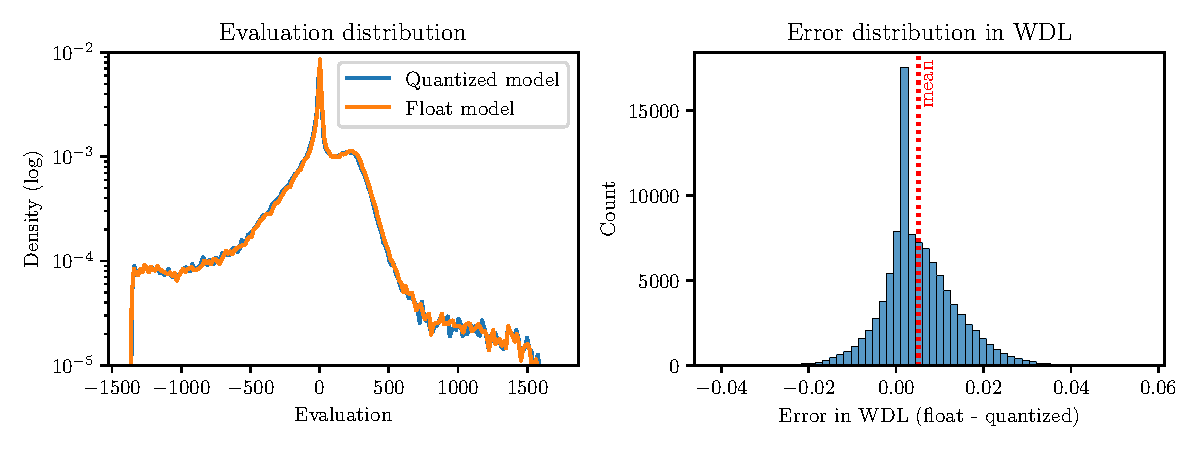
\includegraphics[width=\textwidth]{./dynamic/output/quant_errors.pdf}
\caption{Comparison between the float model and the quantized model. $N=100000$}
\label{fig:quant_errors}
\end{figure}

In Figure \ref{fig:quant_errors} we can see that the distribution of the evaluation of both models is almost identical, indicating that the implementation is correct.

To measure the error introduced it is better to do it in WDL-space, since we can make sense of values in that space. The errors are near zero, and almost all errors are within 0.03 units, which is a 3\% difference in winrate. The Stockfish team has reported that errors in quantization up to 5\% do not affect the engine's strength \footnote{\href{https://discord.com/channels/435943710472011776/718853716266188890/814260897040039977}{Sopel's message on Discord about this} (official Stockfish server).}.

\section{Training}

Given a feature set, the network architecture is completely defined, along with how to encode a position into its inputs. This section will describe two proposed methods to train the networks, each with its own loss function and training dataset.

\subsection{Source dataset}

Data is needed to train the network. The proposal for the thesis was to use the Lichess database \cite{lichessdb}, which provides a CC0 database with all the games ever played on the site, then score the positions using Stockfish. After some initial experiments, the networks were not performing as expected. Upon further reaserch, I found out that I was working with datasets too small for this task (order of hundreds of millions). I needed a larger dataset (order of \textbf{dozens of billions}), but it was impractical for me to generate it. Fortunately, I can use the same dataset that Stockfish uses to train its networks \cite{sf_nnue_dataset}, which should work well. Specifically, I went with the dataset used to train the first stage of the main network for Stockfish 16.1, which is 135GB of compressed \texttt{binpack} files. It was built by running Stockfish at 5000 nodes per move on multiple opening books\footnote{An opening book is a database of start positions (lines of play) generated with some criteria.}. Later stages use datasets generated by Leela Chess Zero (LC0), which is more expensive to compute but has higher quality evaluations.

The \texttt{binpack} format is a very efficient method of storing samples yet very complex to decode. Fortunately, Stockfish provides a tool to export this data into a text representation. I had to modify it to export it in the format I wanted. I changed the \texttt{emitPlainEntry} function in \texttt{nnue\_data\_binpack\_format.h} to the code in Appendix \ref{appendix:emitPlainEntry}. The resulting file was 2.59 terabytes in size and contained \textbf{48.4 billion samples}. There is one sample per line with the format:

\begin{center}
\begin{tabular}{|cp{0.0005cm}cp{0.0005cm}c|}
\hline
\textbf{FEN\footnotemark} & , & \textbf{Score} & , & \textbf{Best move} \\
\hline
\end{tabular}
\end{center}

\footnotetext{Standard notation to describe positions of a chess game. It is a sequence of ASCII characters.}

The file was too big to be practical, and it would wear off my SSD, so I made a tool to compact the data into a similar format. The new format exploits the fact that samples in a row belong to the same game. This means that contiguous FENs are a move from a previous one, so it stores the move instead of the FEN:

\begin{center}
\begin{tabular}{|cp{0.0005cm}cp{0.0005cm}c|}
\hline
\textbf{FEN} & , & \textbf{Score} & , & \textbf{Best move} \\
\hline
\end{tabular}
(
\begin{tabular}{|p{0.0005cm}cp{0.0005cm}cp{0.0005cm}c|}
\hline
, & \textbf{Actual move} & , & \textbf{Score} & , & \textbf{Best move} \\
\hline
\end{tabular}
) *\footnote{Repeated zero or more times.}
\end{center}

As you can see, the new format is compatible with the last one, so only one reader was implemented. After compacting the data, the file went down to a manageable 522 gigabytes. Also, reading a single FEN and later applying moves to it is much faster than parsing a FEN every time. \\

There are many positions in the dataset that are known to not be good for training. Remember that the engine is doing quiescent search, so it does a smaller search looking for quiet positions to evaluate. This means that positions where the \enquote{best} move is a capture, or there is a check, are filtered out when building the training batch. \\

Each training method will generate a new derived dataset based on these samples.

% Lichess is a free online site to play chess, and thankfully it provides a CC0 database \cite{lichessdb} with all the games ever played on the site. It consists of serveral compressed PGN files\footnote{Portable Game Notation: a textual format to store chess games (moves and metadata)} splitted by month since 2013, that add up to $1.71$TB compressed. The whole database contains over 5.5 billion games, that equates to around 200 billion positions. In practice, that many positions are too much to handle so I'll use only a fraction of them and take only one sample per game to increase the diversity of positions.

% The Lichess database also provides a database of puzzles
% hablar de esto en otro lado (results? eval?)

% A single game can have lots of positions, most of which are shared with millions of other games, mostly during the early game. This is a problem of its own: trying to sample positions from a game with a suitable distribution. In this work, I have chosen to only consider positions 20 half-moves into the game.

\subsection{Method 1: Score target}

The main method to train the network will use the scores provided in the dataset as targets. I expect the networks to learn to predict the evaluation of a position as Stockfish would do.

\setcounter{secnumdepth}{4}
\subsubsection{Score-space to WDL-space}

Evaluations in the dataset are values ranging from -10000 to 10000. We call this range of values the score-space, also referred to as the \textit{centipawn scale} (or something proportional to it). We want the network to output the same values as the dataset, in \textit{score-space}.

The WDL-space is a different scale in [0, 1] where 0 is a loss, 0.5 is a draw, and 1 is a win. The WDL (win-draw-loss) model \cite{wdl-model} states that the win rate for a position can be modeled as a function of the evaluation of the position. The data shows that the logistic function (sigmoid) gives a good approximation for the evaluation $f(P)$:

\[
\mathcal{W}(f(P)) = \sigma\left(\frac{f(P)-a}{b}\right) = \frac{1}{1 + e^{-\frac{f(P)-a}{b}}}
\]

where $a$ and $b$ need to be fitted to the data. The value of $a$ is the evaluation where a 50\% winrate is observed, and $b$ indicates how fast the winrate changes when the evaluation change. The fitted sigmoid is shown in figure \ref{wdl-fit}, and the values obtained are $a=1.28$ and $b=297.21$.

\begin{figure}[H]
\centering
\makebox[\textwidth]{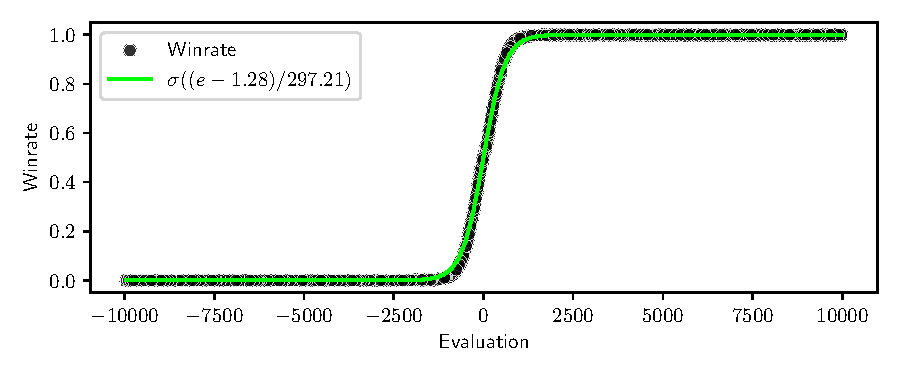
\includegraphics[width=\textwidth]{../assets/sigmoid_fit.pdf}}
\caption{WDL model function (sigmoid) fitted to 100 million evaluations in the dataset.}
\label{wdl-fit}
\end{figure}


During training, it is better to use a loss function with the target and output of the model in WDL-space instead of score-space. WDL-space has some advantages over score-space:

\begin{itemize}
\item Large evaluations are \enquote{closer} together in WDL-space, since having a score of 7500 or 8000 is not that different in terms of winrate (less than 1\%) than between 50 and 550 (more than 30\%). This is desirable because the evaluations do not need to be that precise when the outcome of the game is almost decided.
\item The result of a game can be interpolated in WDL-space. If we introduce a new parameter $\lambda$, we can interpolate the evaluation $f(P)$ and the game result $r$ (in WDL-space) using: $\lambda \cdot \mathcal{W}(f(P)) + (1 - \lambda) \cdot r$. This way, the information about the outcome of the game can be used to steer the network in the right direction. This is not implemented in this work.
\item Values in WDL-space are smaller than in score-space, so it avoids large gradients.
\end{itemize}




\subsubsection{Loss function}

The loss function chosen is mean squared error (MSE) with a power of 2.6 (the value used by the Stockfish's official trainer) given by

% q = (output / out_scaling).sigmoid()
% p = (target / in_scaling).sigmoid()
% loss = torch.pow(torch.abs(p - q), 2.6).mean()

\[
\mathcal{L}(y,f(x,\bm{W}))= \frac{1}{N} \sum_i^N \left| \mathcal{W}(y_i) - \mathcal{W}(f(x_i,\bm{W})) \right| ^{2.6}
\]

where\dots

\begin{enumerate}
\itemsep0em
\item $N$ is the number of samples.
\item $y$ are the target scores.
\item $f$ is the model.
\item $x$ are the inputs (encoded feature sets).
\item $\bm{W}$ are the parameters of the model.
\item $\mathcal{W}$ is the winrate function that maps from score-space to WDL-space.
\end{enumerate}

\subsection{Method 2: PQR triplets}

This is an additional technique I wanted to try, described in \cite{dlchess:2014}. The method is based on the assumption that moves in the training data are better than random. In the blog they used human moves from the Lichess database \cite{lichessdb}, so they rely on the fact that humans make good or near-optimal moves most of the time, even if they are amateurs. In my case, I will use Stockfish moves, which are extremely good. This method does not use the scores provided; it will have to learn them from scratch. Of course this is way harder to train, but I'm curious to see how far the following idea can go.

Remember that we are trying to obtain a function $f$ (the model) to give an evaluation of a position. The idea is based on the following two principles:

\begin{enumerate}
\item For two positions in succession $P \rightarrow Q$ observed in a game, we will have \mbox{$f(P)=-f(Q)$}. This comes from the fact that the game is zero-sum.
\item Going from the position $P$, not to the observed position $Q$, but to a \textit{random} position $P \rightarrow R$, we must have $f(R) > f(Q)$ because the random move is better for the next player and worse for the player that made the move.
\end{enumerate}

If these reasonable assumptions hold, a loss function that expresses the equality in (1) and the inequality in (2) can be constructed.

% Consider an optimal $f$, that outputs $-1,0,1$ depending on who wins.
% With infinite compute, $f$ would be the result of running minimax to the end of the game, since minimax always finds optimal moves.

\subsubsection{Loss function}

The loss function is the sum of the negative log-likelihood of the inequalities: ${f(R) > f(Q)}$, ${f(P) > - f(Q)}$ and ${f(P) < -f(Q)}$. The last two are a way to express the equality \mbox{$f(P)=-f(Q)$}. Each term is the negative log-likelihood function of the known Bradley-Terry model \cite{bradley-terry:1952}, that models the probability of an item (in our case a position) \enquote{beating} another item.

The loss function is given by

\begin{align*}
\mathcal{L}(x^P, x^Q, x^R, \bm{W})=
\frac{1}{N}
\sum_i^N
& -\log\left(\sigma(r_i - q_i)\right) \\
& -\log\left(\sigma(p_i + q_i)\right) \\
& -\log\left(\sigma(-(p_i + q_i))\right)
\end{align*}

where\dots

\begin{enumerate}
\itemsep0em
\item $N$ is the number of samples.
\item $x^i$ are the inputs (encoded feature sets) for the $i \in \{P,Q,R\}$ positions.
\item $f$ is the model.
\item $\bm{W}$ are the parameters of the model.
\item $\mathcal{W}$ is the winrate function that maps from score-space to WDL-space.
\item $\overline{\mathcal{W}}(x) = 2 \mathcal{W}(x) - 1$ is a function that maps from WDL-space [0, 1] to $[-1, 1]$, so that $\overline{\mathcal{W}}(x) = -\overline{\mathcal{W}}(-x)$.
\item $
p_i = \overline{\mathcal{W}}(f(x^P_i, \bm{W})),\text{ }
q_i = \overline{\mathcal{W}}(f(x^Q_i, \bm{W}),\text{ }
r_i = \overline{\mathcal{W}}(f(x^R_i, \bm{W})
$. Note that quantization is happening in this method too, so the output of the model is being scaled appropriately.
\end{enumerate}



Let's break down the loss function in a more intuitive way. We want the loss function to be small when the model is generating the correct evaluations and large when it is not. Let's look at the graph of the function $-\log(\sigma(x))$:

\begin{figure}[H]
\centering
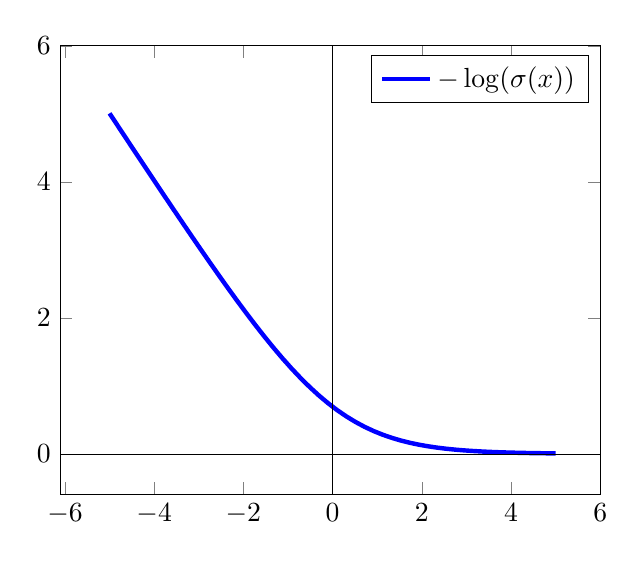
\begin{tikzpicture}
\begin{axis}[xmax=6,ymax=6, samples=50]
\addplot[blue, ultra thick] (x,{-ln(1/(1+e^-x))});
\draw[ultra thin] (axis cs:\pgfkeysvalueof{/pgfplots/xmin},0) -- (axis cs:\pgfkeysvalueof{/pgfplots/xmax},0);
\draw[ultra thin] (axis cs:0,\pgfkeysvalueof{/pgfplots/ymin}) -- (axis cs:0,\pgfkeysvalueof{/pgfplots/ymax});
\addlegendentry{$-\log(\sigma(x))$}
\end{axis}
\end{tikzpicture}
\end{figure}

The function approaches 0 when $x$ grows and approaches $\infty$ when $x$ goes to $-\infty$.

Let's look at each of the terms:

\begin{enumerate}
\itemsep0em
\item $-\log(\sigma(r_i - q_i))$: This term is small when $r_i > q_i$, and large when $r_i < q_i$.
\item $-\log(\sigma(p_i + q_i))$: This term is small when $p_i > -q_i$, and large when $p_i < -q_i$.
\item $-\log(\sigma(-(p_i + q_i))$: This term is small when $p_i < -q_i$, and large when $p_i > -q_i$.
\end{enumerate}

The term (1) holds the inequality $f(R) > f(Q)$, and the terms (2) and (3) hold the equality $f(P) = -f(Q)$. The loss function is the sum of the three terms, so the model is encouraged when it satisfies the inequalities and penalized when it does not.

\subsection{Setup}


The project is written in two languages: Rust and Python. The Rust part is used to process dataset files, generate statistics, and provide final training batches for Python to consume. The Python part defines the Pytorch model, runs the training loop, quantizes the model, and runs the evaluations. \\

The training process is started by running a Python script (\texttt{scrips/train.py}) and it requires to define the model architecture (number of neurons on each layer), general training parameters (learning rate, batch size, epochs, checkpoints, etc.) and the feature set to use, which in turn determines the size of the batches. For example, if PQR is used, the size of a sample is three times the size of the feature set times two (because it is siamese), and if it is score target, it is the size of the feature set times two plus one for the target score.

To orchestrate training runs, the platform Weights and Biases (WandB) is used. It provides automatic sweeping of hyperparameters, logging of metrics, and visualizations. Results are exported from the platform in CSV and then processed by Python scripts. \\

The training data has to be converted to an actual tensor of floats to be consumed by Pytorch. This is done by a Rust subprocess running the subcommand \texttt{batch-loader} that reads the training data file and generates training batches for the specified feature set in a shared memory buffer.

The batch generation process is heavily parallelized. Let's call $N$ the number of threads ($N=8$ was used). When the process starts, it splits the dataset file into $N$ equal parts and assigns each part to a thread. Each thread reads samples sequentially and builds the batch in a buffer. The buffer is then sent to the main thread, where it is copied to the shared memory buffer.

The Python script copies the data from the shared buffer at the start of each iteration, allowing Rust to generate the next batch (in the CPU) while Pytorch is training the current batch (in the GPU). To coordinate the memory access between the two processes, a single byte is sent using standard I/O. The sequence of a training loop is shown in figure \ref{training-loop}.

\begin{figure}[H]
\centering
\makebox[\textwidth]{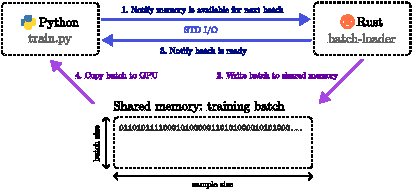
\includegraphics[width=\textwidth]{../assets/training-loop.pdf}}
\caption{Sequence of steps to send a batch from the \texttt{batch-loader} subprocess in Rust to Pytorch.}
\label{training-loop}
\end{figure}

Given that the input vector is multiple-hot encoded, the data written by the Rust process are not float values. Instead, they are 64-bit integers acting as a bitset. Before passing the vector to the model, it is expanded into floats. This means 64 floats can be packed into a single 64-bit integer, meaning a \textbf{96.875\%} reduction in memory usage (from 256 to 8 bytes). The speedup obtained by this optimization was substantial. The compression can be further improved using sparse tensors, but it is not implemented in this work. \\

%\begin{figure}[H]
%\centering
%\makebox[\textwidth]{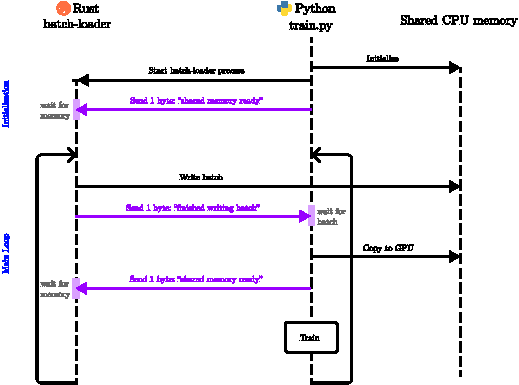
\includegraphics[width=\textwidth]{../%assets/training.pdf}}
%\caption{assad.}
%\end{figure}

% [evaluation?]
% [a esta seccion se le pueden agregar mil cosas]
% [multithreaded, perf]
% decir que en "All" tengo 450 it/s (7.3M pos/sec)


\newcommand{\depiction}[1]{\parbox{0.7cm}{\includegraphics[height=0.7cm]{../assets/depictions/#1.pdf}}}
\newcommand{\depictionSM}[1]{\parbox{0.6cm}{\includegraphics[height=0.6cm]{../assets/depictions/#1.pdf}}}


\section{Experiments and results}

Now that the engine, the tools and the methodology are defined, we can proceed to the experiments. Experiments will be divided in three sections: motivation, experiment and results. The motivation will explain why I think the experiment is relevant and present possible hypothesis. The experiment will describe configurations to train different models, how they will be evaluated and what are my expectations. The results will present the data, explain whether my hypothesis was correct or not and give a brief conclusion. \\

Every model's training configuration is defined by the following variables:

\begin{itemize}
\item \textbf{Feature set}: Determinates the encoding of the position, and thus the number of inputs of the model. It conditions which patterns the network can learn. Experimenting with this is the main focus of this thesis.

\item \textbf{Network architecture}: The size of each layer in the network. The first layer (L1) is the feature transformer and it is efficiently updated. The following layer (L2) should be tiny due the NNUE architecture. The size of the model (its complexity) roughly determinates how many patterns the network can learn.

\item \textbf{Dataset}: The positions to train on. The dataset used is explained in detail in chapter 5. In summary, there are 48.5 billion positions to train on and the dataset remains constant across all runs. About 5 million positions are used for validation.

% no me gusta la palabra computed...
\item \textbf{Training method}: Can choose to use either score targets or PQR triplets. This determinates the format of the samples as well as the loss function. All experiments will train using score targets, unless specified. Methods were explained in detail in chapter 5.

\item \textbf{Training hyperparameters}: The usual machine learning hyperparameters for training, such as batch size, learning rate and scheduler. Recall that each epoch is 100 million positions, and the training will last for 256 epochs (25.6 billion positions).
\end{itemize}

Once training is completed, the models will be evaluated depending on the experiment. To assess the performance of a model or to compare a set of models, the following indicators are used:

\begin{itemize}
\item \textbf{Loss}: The training and validation loss are used to detect overfitting and other possible problems. It can't be used to measure the performance of a model. Bigger models must have much better predictions to outweight the cost of having slower inferences and thus less node visits. It's a tradeoff.

\item \textbf{Puzzle accuracy}: The percentage of moves correctly predicted by the engine in Lichess puzzles. Each puzzle may contain multiple moves, and the engine has 100ms per move. Since the engine is not that strong, it does not solve 100\% of puzzles like many other engines do, so I expect differences in this metric to be good indicators. A small set of puzzles is used during training as (a very bad) proxy for the engine's strength, to have early insight of the strength and to detect catastrophic failures that did arise. A bigger set of 85000 puzzles is used after training.

\item \textbf{Relative ELO rating}: A tournament is played between different models to determine their relative strength. Ordo is used to compute the ELO of each model based on the results of the tournament. This is the most important metric, as it is the most reliable way to compare the strength of engines.

% \item \textbf{Inference performance (infs/s)}:

\item \textbf{Training duration}: The amount of time it takes to train a model. This is a one time operation and it does not affect the performance of a model. However, it does condition which and how many experiments I can run.
\end{itemize}

All networks that are not in the first experiment (the baseline), are trained 4 times and a tournament is played between the epoch 192 and 256 of each network (8 networks in total). I have observed a difference of 30 elo points between runs, so this step is crucial to have sensible results. In the appendix are the results of each run and tournament. \\

The experiments are all run in the same hardware: Intel 14900K CPU (24 cores, 32 threads) for dataset generation, batching and evaluation, and a single NVIDIA RTX 4090 24GB GPU for training.

\subsection{Baseline}

\textbf{Motivation.} Experiments that will follow will focus on trying out different feature sets, so it is natural to keep every other variable constant. Since the dataset is fixed and the feature set is going to be changing, it remains to find acceptable values for the network architecture and the training hyperparameters. 

Due time and resources constraints, I decided to set the training hyperparameters to   (similar) values which give good results in the official Stockfish trainer: \textbf{a batch size of 16384, a learning rate of 0.0005 and a exponential decay factor of 0.99}. This values showed acceptable results during early stages of development and will remain fixed for all runs.

It remains to find a good network architecture. Bigger networks may have lower loss and predict better, but they will also have slower inferences. This is the tradeoff between inference time and node visits (more depth), which are also affected by the quality of the prediction due to better pruning. So the model must be so much better to compensate the slowdown in inference. \\

\textbf{Experiment.}  In this first experiment I will try different sizes of L1 and L2,  to find an acceptable tradeoff for future experiments. I will run a grid search with L1 $\in \{256, 512, 1024, 2048\}$ and L2 $\in \{32, 64, 128, 256\}$. The feature set used to train will be \featureset{All}, the canonical set with 768 features.

I expect that there will be a model that performs best and other models that are smaller (need stronger predictions) and bigger (need speed to visit more nodes) perform worse. \\

\textbf{Results.} Looking at the result heatmaps in Figure \ref{fig:baseline_heatmaps}, the first thing to notice is that training and validation losses behave as expected. If the model is more complex, meaning the number of parameters (which is dominated by $768*L1+L1*L2$) is higher, the loss is lower and the model predicts better.

When the models are loaded into the engine and evaluated in a tournament, we can see that when L2 drops, the performance drops dramatically. This is due the fact that the inference time is mostly dominated by L2. This result suggests that it may be a good idea explore even lower values of L2, such as 16 or even 8. However, the SIMD implementation requires L2 to be a multiple of 32 so it needs a refactor to keep being fast. So, instead of fiddling further with SIMD I decided to \textbf{keep L2 at 32}.

\begin{figure}[H]
\centering
\makebox[\textwidth]{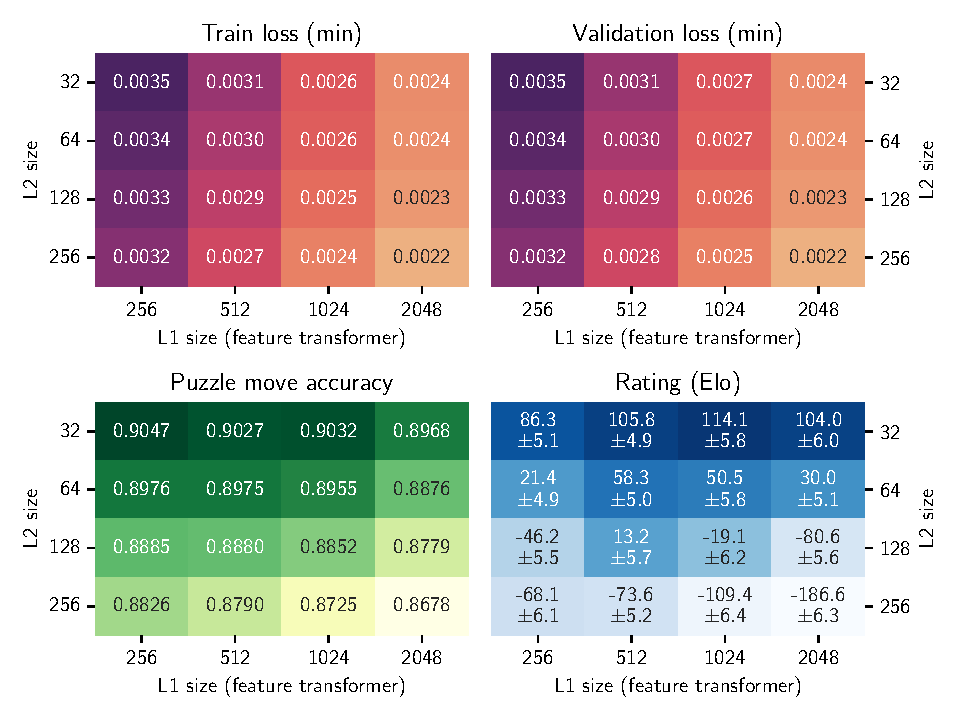
\includegraphics[width=\textwidth]{./dynamic/output/baseline_heatmaps.pdf}}
\captionsetup{justification=centering}
\caption{Network architecture sweep results (L1 $\times$ L2).\\ Table with details in Appendix \ref{appendix:baseline}.}
\label{fig:baseline_heatmaps}
\end{figure}

If L2 is kept constant, the best L1 is not the smallest nor biggest. If L2 $=64$ or L2 $=128$ there is a clear lead of L1 $=512$ in both. In the case of L2 $=32$, the best L1 is not clear because the differences in rating are small and are within margin of error, excluding L1 $=256$ which is definitely wrose. Because training lower values of L1 is faster I opted for \textbf{L1} $\bm{=512}$ due the difference being small and being the best in other L2 values.

So, further experiments will use L1 $=512$ and L2 $=32$. For reference, Stockfish currently uses L1=2560, and employ (lots of) more tricks to make it even faster. The values selected here are specific to the current implementation of the engine, since it may change if more optimizations are made (tradeoff is altered). For this reason, no further modifications to the engine were made after starting with the experiments. We can now proceed with more interesting experiments.

\subsection{Axis encodings}
\label{sec:axis_encoding}

\textbf{Motivation.} Looking back at the networks generated by \featureset{All} in baseline runs, the learned weigths of most neurons in the feature transformer layer (L1) are related with the movement pattern of the pieces. Let's take the example in Figure \ref{fig:rook_weights}, which depicts the \featureset{Square} part of the features where the role is \symrook\ Rook.

\begin{figure}[h]
\centering
\subfloat[\centering $\white$ White]{{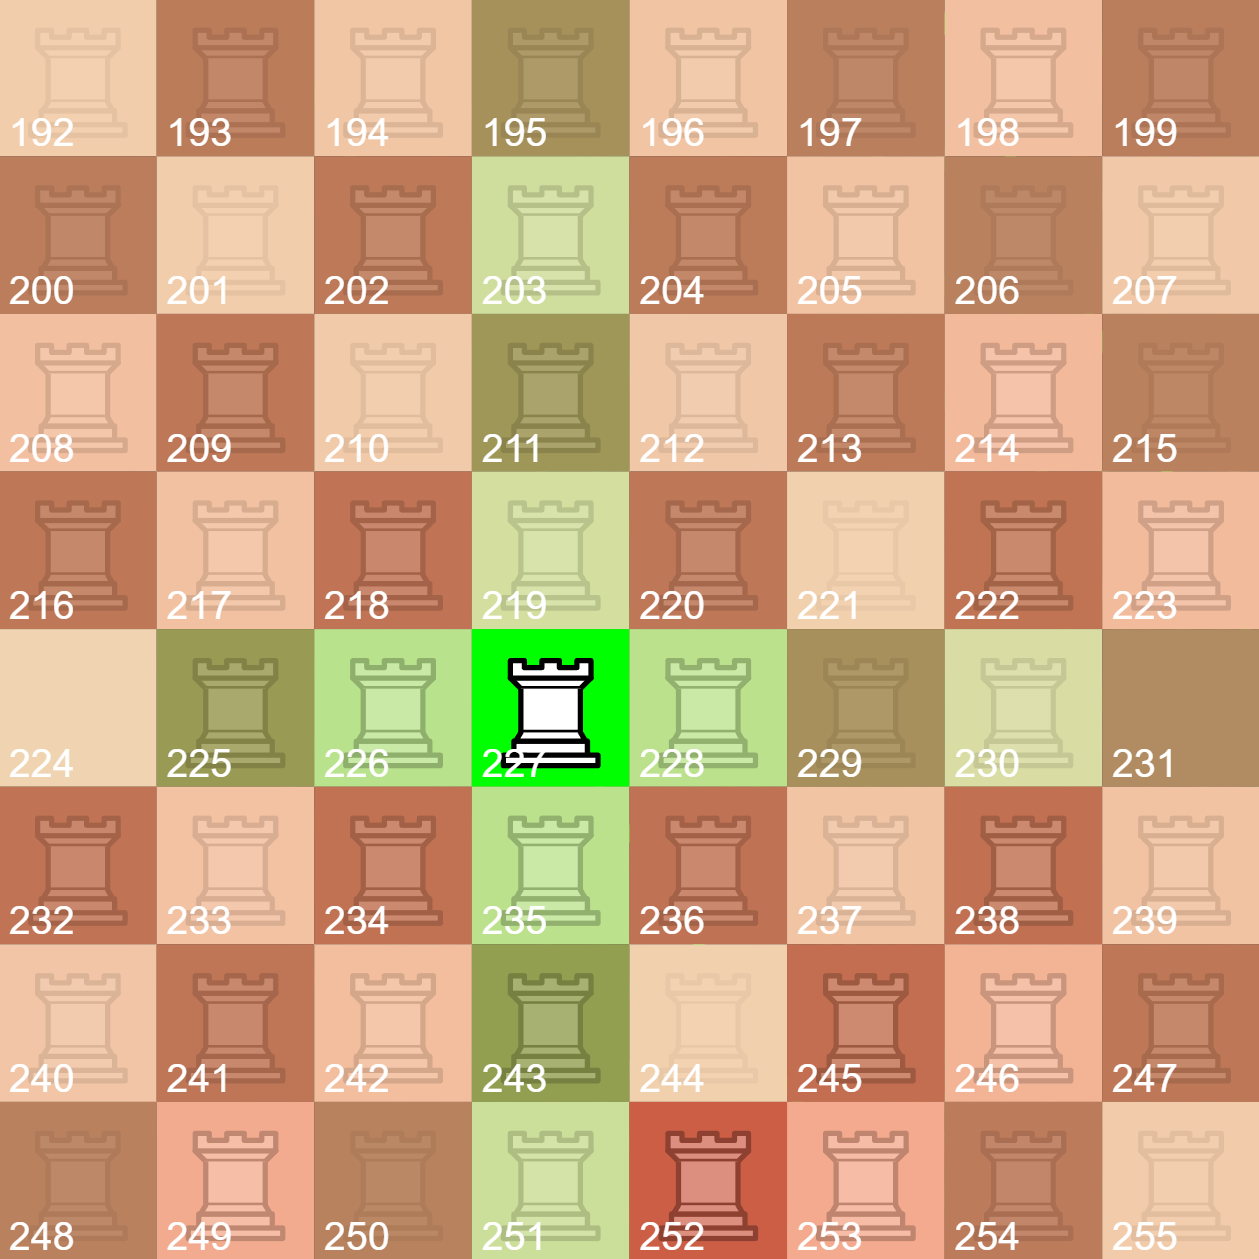
\includegraphics[width=7cm]{../assets/results/piece_weights/white_rook_weights.png} }}%
\qquad
\subfloat[\centering $\black$ Black]{{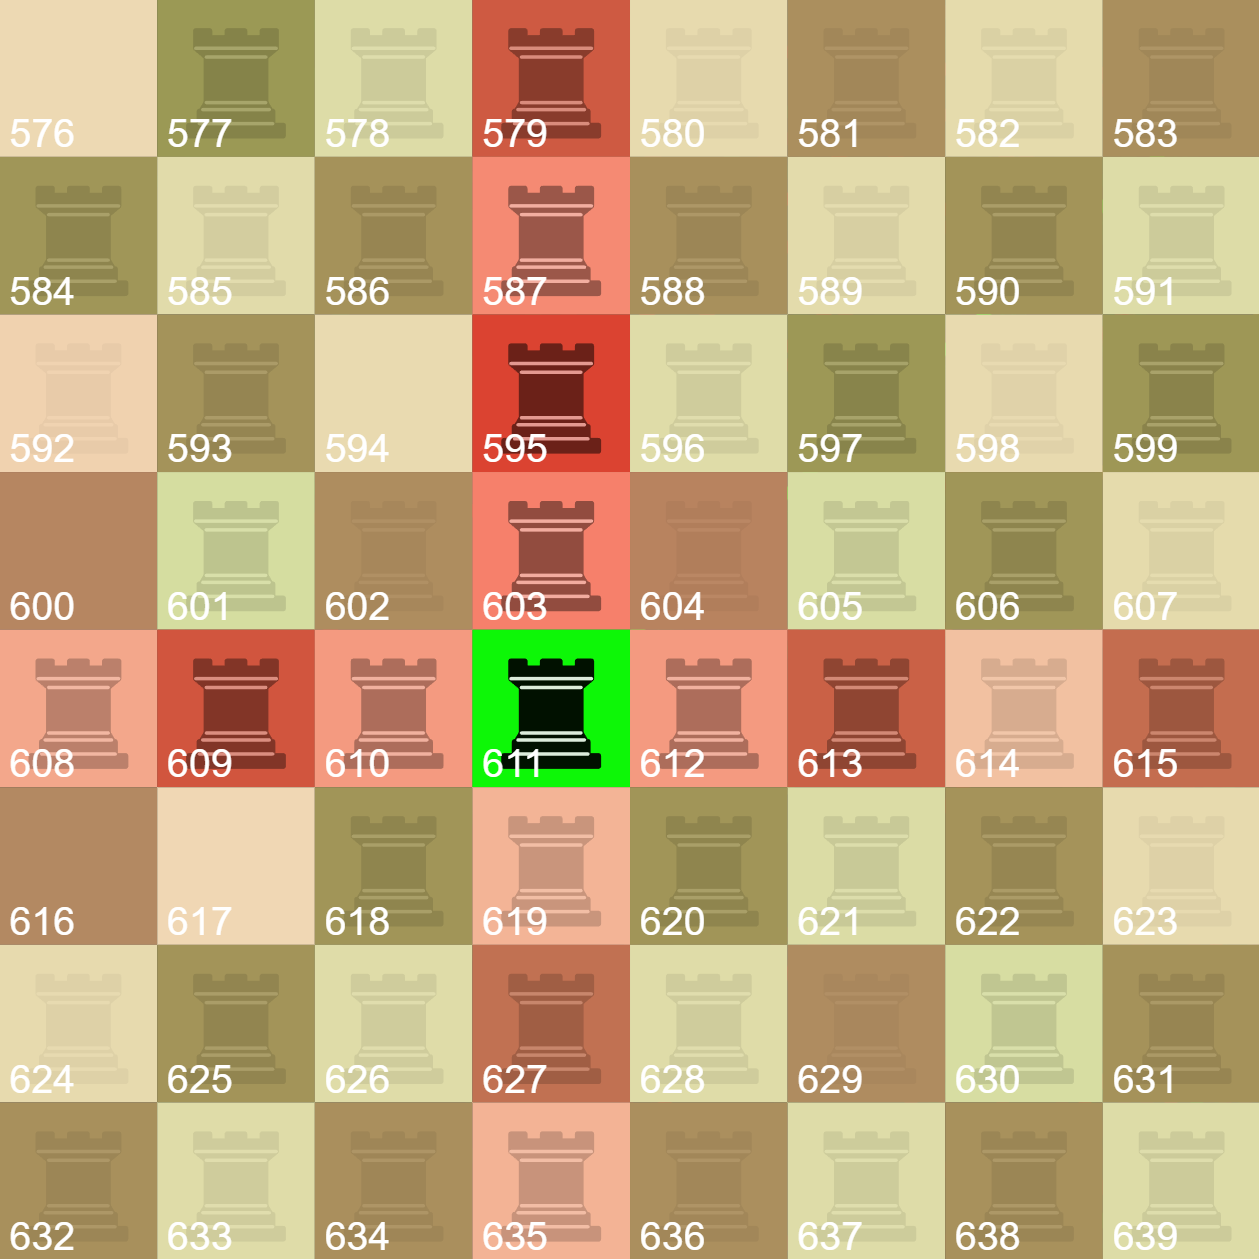
\includegraphics[width=7cm]{../assets/results/piece_weights/black_rook_weights.png} }}%
\caption{Weights of \textbf{a neuron} in the L1 layer, which are connected to features in \featureset{All} where the role is $\rook$ Rook. The intensity represents the weight value, and the color represents the sign (although not relevant).}
\label{fig:rook_weights}
\end{figure}

This particular neuron learned to recognize the presence of a \symrook\ Rook, affected by the pattern of another potential rook in the same file or rank (other pieces may be involved but I am focusing on rooks for the example). Doing so, it had to relate one feature for every potential square where a rook could be for that specific center location, which restrains the network from learning more complex patterns and it is harder to train, because you need more samples to account for all possible combinations.

What if we add a feature which describes \enquote{\textit{there is a $\white$ White $\rook$ Rook in the 4th rank}}? Certainly, this would make the network's job easier, as it would only need to learn the presence of rooks in the corresponding file or rank, instead of every square. This idea can be extrapolated to diagonals, to ease patterns with $\bishop$ Bishops and the $\queen$ Queen.

More examples of this behaviour can be found in Appendix \ref{appendix:axis_samples}, showcasing diagonal patterns and the $\knight$ Knight movements, although they do not move straight through axes. \\

\textbf{Experiment.} I built blocks of features for each natural axis of a chess board, which coincide with the movement pattern of the pieces:

\begin{table}[H]
\centering
\begin{tabular}{cccc}
\depiction{H} & \depiction{V} & \depiction{D1} & \depiction{D2} \\
Horizontal & Vertical & Diagonal 1 & Diagonal 2 \\
(across files) & (across ranks) &  & 
\end{tabular}
\end{table}

% The canonical \featureset{All} feature set encodes each piece's position using the square it is located. Note that this is the same thing as encoding the position for a piece $P$ as $\featureset{File}_{P} \times \featureset{Rank}_{P}$. So the position of each piece is determined using the vertical (across ranks) and horizonal (across files) axes.

In table \ref{tab:axes_blocks} I present the feature blocks. Each block will encode whether there is a piece with the role and color in a specific location along that axis, as explained in the example.

\begin{table}[H]
\caption{Axes feature blocks}
\label{tab:axes_blocks}
\centering

\newcommand{\fullrolecolor}{$\times$ $\featureset{Role}_{P} \times \featureset{Color}_{P}$}

\begin{tabular}{cccccc}
\toprule
\bf Depiction & \bf Block name & \multicolumn{2}{c}{\makecell{\bf Definition\\for every piece $P$ in the board}} & \bf \makecell{Number of\\features} \\
\toprule
\depiction{H} & $\featureset{H}$ & $\featureset{File}_{P}$ & \fullrolecolor & 96 \\
\depiction{V} & $\featureset{V}$ & $\featureset{Rank}_{P}$ & \fullrolecolor & 96 \\
\depiction{D1} & $\featureset{D1}$ & $\featureset{Diag1}_{P}$ & \fullrolecolor & 180 \\
\depiction{D2} & $\featureset{D2}$ & $\featureset{Diag2}_{P}$ & \fullrolecolor & 180 \\
\bottomrule
\end{tabular}

\end{table}


With this blocks, I built different feature sets (listed in table \ref{tab:axis_encoding}): one group of feature sets is just combinations of all the blocks, and another group which is the same as the first but alongside the \featureset{All} feature set (here treated as a block). The second group is the aim of the experiment, it has the classic \featureset{All} feature set but includes the axis blocks to see if the network can benefit from them. The first group, which does not include \featureset{All} is to know how far the network can go only with this blocks alone.

\begin{table}[H]
\caption{Axis encodings feature sets}
\label{tab:axis_encoding}
\centering

\newcommand{\rolecolor}{$\times$ $\featureset{R}_{P} \times \featureset{C}_{P}$}

\begin{tabular}{ccc}
\toprule
\bf Depiction & \bf Feature set & \bf \makecell{Number of\\features} \\
\toprule
\depiction{H} $\oplus$ \depiction{V} & $\featureset{H} \oplus \featureset{V}$ & 192 \\
\midrule
\depiction{D1} $\oplus$ \depiction{D2} & $\featureset{D1} \oplus \featureset{D2}$ & 360 \\
\midrule
\depiction{H} $\oplus$ \depiction{V} $\oplus$ \depiction{D1} $\oplus$ \depiction{D2} & $\featureset{H} \oplus \featureset{V}$ $\oplus$ $\featureset{D1} \oplus \featureset{D2}$ & 552 \\
\midrule
% ------------------------------------
\midrule
\featureset{All} $\oplus$ \depiction{H} $\oplus$ \depiction{V} & $\featureset{All} \oplus \featureset{H} \oplus \featureset{V}$ & 960 \\
\midrule
\featureset{All} $\oplus$ \depiction{D1} $\oplus$ \depiction{D2} & $\featureset{All} \oplus \featureset{D1} \oplus \featureset{D2}$ & 1128 \\
\midrule
\featureset{All} $\oplus$ \depiction{H} $\oplus$ \depiction{V} $\oplus$ \depiction{D1} $\oplus$ \depiction{D2} & \featureset{All} $\oplus$ \featureset{H} $\oplus$ \featureset{V} $\oplus$ \featureset{D1} $\oplus$ \featureset{D2} & 1320 \\
\bottomrule

\end{tabular}
\end{table}

I expect that the feature sets that are sums of single axes ($\depictionSM{H} \oplus \depictionSM{V}, \depictionSM{D1} \oplus \depictionSM{D2}$ and $\depictionSM{H} \oplus \depictionSM{V} \oplus \depictionSM{D1} \oplus \depictionSM{D2}$) will perform worse overall, since to capture the exact position of pieces in the board, the network will have to learn to relate at least two features for every location. This information is already available when \featureset{All} is present.

The feature sets that include \featureset{All} (\featureset{All} $\oplus \hdots$) should perform better than without, providing that the idea explained in the motivation holds.

For each of the proposed feature sets, I will train a network and evaluate its performance relative to each other using a tournament. I expect to see them ranked in the reverse order as presented in the table (more extra axes better). \\

\textbf{Results.} The results in table \ref{tab:axis_results} show that indeed, adding the axes blocks make the network validation loss slightly lower, from 0.00316 in \featureset{All} to 0.00307 including all four blocks. However, this improvement in loss is not significant enough to make the network stronger to compensate the (small) performance hit of having more features. As you can see in the table, including more axes makes the loss decrease slightly yet the rating decreases by a huge factor.

All three feature sets that do not include \featureset{All} unsuprisingly perform much, much worse even having less features. The feature set \featureset{H+V+D1+D2} has a 25\% higher loss than \featureset{All} and $172.5 \pm 4.8$ less rating than \featureset{All}. The other feature sets in this group perform even worse, as it was expected.

I discovered that the accuracy of puzzles is not a good a proxy of an engine's strength, given that there is a 474 rating difference yet 3\% a difference in move accuracy. I believe that the reason lies on the fact that puzzles may be more strategic than positional. I will drop the puzzle accuracy metric in future experiments.

\begin{table}[H]
\caption{Axis encodings results}
\label{tab:axis_results}
\centering

% 1 256-eval_16384_(hv[768]→512)x2→32→1.nn          :     0.0   ----  22665.5   32456    70      96
% 2 256-eval_16384_(hv+h+v[960]→512)x2→32→1.nn      :    -4.6    5.0  22474.0   32456    69     100
% 3 256-eval_16384_(hv+d1+d2[1128]→512)x2→32→1.nn   :   -33.3    5.0  21260.5   32456    66     100
% 4 256-eval_16384_(hv+h+v+d1+d2[1320]→512)x2→32→1.nn   :   -57.7    4.8  20207.5   32458    62     100
% 5 256-eval_16384_(h+v+d1+d2[552]→512)x2→32→1.nn   :  -172.5    4.8  15176.0   32456    47     100
% 6 256-eval_16384_(h+v[192]→512)x2→32→1.nn         :  -368.1    5.7   7527.0   32460    23     100
% 7 256-eval_16384_(d1+d2[360]→512)x2→32→1.nn       :  -474.5    6.4   4289.5   32458    13     ---

% Network: 256-eval_16384_(d1+d2[360]→512)x2→32→1.nn Accuracy: 0.851789055191768
% Network: 256-eval_16384_(h+v+d1+d2[552]→512)x2→32→1.nn Accuracy: 0.8748684518241348
% Network: 256-eval_16384_(h+v[192]→512)x2→32→1.nn Accuracy: 0.8618817235734331
% Network: 256-eval_16384_(hv+d1+d2[1128]→512)x2→32→1.nn Accuracy: 0.8814458606173995
% Network: 256-eval_16384_(hv+h+v+d1+d2[1320]→512)x2→32→1.nn Accuracy: 0.8766955098222639
% Network: 256-eval_16384_(hv[768]→512)x2→32→1.nn Accuracy: 0.8865762394761459
% Network: 256-eval_16384_(hv+h+v[960]→512)x2→32→1.nn Accuracy: 0.8851511342376053

\begin{tabular}{cccccc}
\toprule
\bf Feature set  & \bf \makecell{Number\\of features} & \makecell{\bf Val. loss\\\textit{min}} & \makecell{\bf Rating\\\textit{elo (rel. to \featureset{All})}} & \makecell{\bf Puzzles\\\textit{move acc.}} \\
\toprule
\depiction{H} $\oplus$ \depiction{V} & 192 & 0.00581 & -368.1 $\pm$ 5.7 & 0.8618 \\
\midrule
\depiction{D1} $\oplus$ \depiction{D2} & 360 & 0.00670 & -474.5 $\pm$ 6.4 & 0.8517 \\
\midrule
\makecell{\depiction{H} $\oplus$ \depiction{V} $\oplus$ \\ \depiction{D1} $\oplus$ \depiction{D2}} & 552 & 0.00389 & -172.5 $\pm$ 4.8 & 0.8748 \\
\midrule
% ------------------------------------
\midrule
\featureset{All} (reference) & 768 & 0.00316 & \textbf{0.0} & 0.8865 \\
\midrule
\featureset{All} $\oplus$ \depiction{H} $\oplus$ \depiction{V} & 960 & 0.00308 & -4.6 $\pm$ 5.0 & 0.8851 \\
\midrule
\featureset{All} $\oplus$ \depiction{D1} $\oplus$ \depiction{D2} & 1128 & 0.00309 & -33.3 $\pm$ 5.0 & 0.8814 \\
\midrule
\makecell{\featureset{All} $\oplus$ \depiction{H} $\oplus$ \depiction{V} \\ \hspace{0.75cm} $\oplus$ \depiction{D1} $\oplus$ \depiction{D2}} & 1320 & \textbf{0.00307} & -57.7 $\pm$ 4.8 & 0.8766 \\
\bottomrule

\end{tabular}
\end{table}

The next experiment will focus on adding more specific features, instead of more broad ones.


\subsection{Pairwise axes}

Pepito \depiction{PH} asdo \depiction{PV} asd\depiction{PD1} asd\depiction{PD2} asd

[explicar...]

3 runs
HV + PH
HV + PV
HV + PH + PV

el cosito de los pares \\

los resultados no son buenos...

I did not bother implementing diagonal pairs.


\noindent\rule{\textwidth}{1pt}

\vspace{0.2cm}
Up to this point, I have been trying to encode the position of the pieces in different or smarter ways, with no avail. It may seem that the network is able to extract all the information it needs from the most basic \featureset{All} feature set. Making the information available in another form makes no difference, as opposed to what I originally thought.

Further experiments will focus on features not related to the position of the pieces, but to other aspects of the game, inspired by hand crafted evaluations.

\noindent\rule{\textwidth}{1pt}


\subsection{Mobility}

\textbf{Motivation.} Mobility in chess is a measure of the available moves a player can make in a given position. The idea is that if a player has more available moves, the position is stronger. In \cite{slater:1950} it was shown that there is a strong correlation between a player's mobility and the number of games won. This metric has been used extensively in hand crafted evaluations, and I propose to include this information as features for the neural network.

There are a couple of ways to go about encoding mobility:

\begin{itemize}
\item \textbf{Bitsets (per piece type):} the amount of features changed each turn may negate any gains.

\begin{figure}[h]
\centering

\begin{tabular}{ccccc}

\raisebox{-7ex}{\chessboard[
    setfen=r5k1/1b1p1ppp/p7/1p1Q4/2p1r3/PP4Pq/BBP2b1P/R4R1K w - - 0 20,
    tinyboard,
    showmover=false,
]}
&

\raisebox{-7ex}{\chessboard[
    tinyboard,
    showmover=false,
    setwhite={ba2,bb2},
    pgfstyle=color,
    opacity=0.8,
    color=blue,
    markfield={b1,c1,c3,d4,e5,f6,g7}
]}

&

\raisebox{-7ex}{\chessboard[
    tinyboard,
    showmover=false,
    addblack={Bb7,Bf2},
    pgfstyle=color,
    opacity=0.8,
    color=blue,
    markfield={c8,c6,d5,a7,b6,c5,d4,e3,e1,g1,g3}
]}

&

\raisebox{-7ex}{\chessboard[
    tinyboard,
    showmover=false,
    setwhite={qd5},
    pgfstyle=color,
    opacity=0.8,
    color=blue,
    markfield={d6,d7,e6,f7,e5,f5,g5,h5,e4,d4,d3,d2,d1,c4,c5,b5,c6,b7}
]}

& $\hdots$

\\

Board &
\makecell{\white White\\\symbishop\ Bishop} &
\makecell{\black Black\\\symbishop\ Bishop} &
\makecell{\white White\\\symqueen\ Queen}

\end{tabular}
\end{figure}


\item \textbf{Counts (per piece type):}
\end{itemize}


\newpage
\subsection{PQR}

\textbf{Motivation.} During the initial research for a thesis subject, I came across \cite{dlchess:2014} which seemed an interesting approach to train a neural network to evaluate positions. Since it was released in 2014, it predates the NNUE era and the training data was suboptimal (Lichess database \cite{lichessdb} with human moves). So I decided to try to replicate the idea using modern datasets, better moves and a proper engine. The \enquote{PQR} method itself was explained in detail in the previous chapter.  Remember that $p$ is a position in the dataset, $q$ is the position obtained by making the best move according to the dataset and $r$ is a random position obtained making a random move from $p$ such that $r \neq q$. \\

Before starting the experiment, I checked if existing networks trained with the conventional method behave under the principles of the PQR method: ${f(p) = -f(q)}$ and ${f(r) > f(q)}$. In the left plot of figure \ref{pqr-eval}, we can see that values of $f(p)$ and $f(q)$ are negatively correlated, which supports the principle that $f(p)=-f(q)$. In the right plot, we can see that the distribution of the difference between $f(r)$ and $f(q)$ is mostly positive, which supports the principle that $f(r) > f(q)$. This shows that the principles that the PQR method relies on are properties that manifest in existing models.

\begin{figure}[H]
\centering
\makebox[\textwidth]{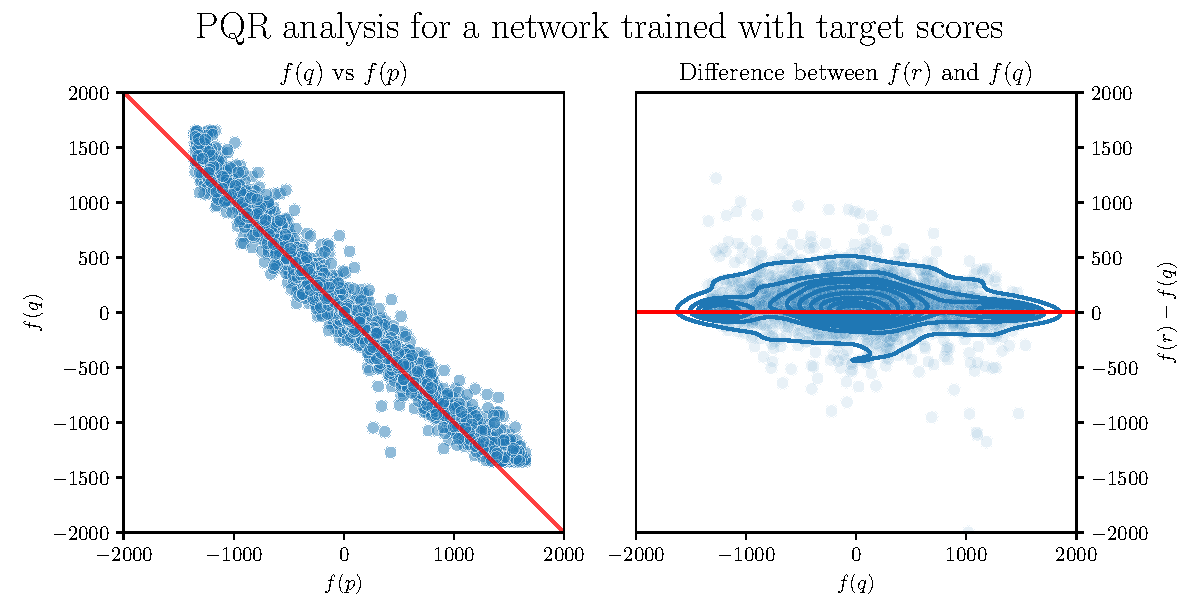
\includegraphics[width=\textwidth]{../dynamic/output/pqr_eval.pdf}}
\caption{Analysis of $N=10000$ PQR positions using a model trained with target scores and the feature set \featureset{All}.}
\label{pqr-eval}
\end{figure}

\textbf{Experiment.} I will train the canonical \featureset{All} feature set with this method in two ways:

\begin{itemize}
\item \textbf{Train from scratch.} The network is initialized with random weights and trained with the PQR method. This is what the original authors did, and I do not expect to reach the performance of models trained with the evaluations method. Using precomputed evaluations as a target is a lot simpler for the model, since it only has to learn to mimic the scores.

\item \textbf{Train from a checkpoint.} A strong checkpoint trained with the other method is used to initialize the network. This way, the network does not have to learn too much at once and may enable it to improve the existing parameters. I believe that two scenarios are likely to happen: the model improves very slowly, or it completely forgets what it have learned before and ends up like a model trained from scratch. The best scenario is that the model improves slowly, proving that it can be used to further optimize existing models.
\end{itemize}

\textbf{Results.}


aqui pondria los resultados... si los tuviera!


%\subsection{Active neurons}
%medir si hay feature sets que no usen neuronas, que esto disparo el uso de HalfTopK
%average number of features enabled by feature set (cantidad y porcentaje)
%measure updates per move average and refreshes average per FS
%[ESTO PONERLO EN EL APPENDIX]


%%%%%%%%%%%%%%%%%%%%%%%%%%%%%%%%%%%%%%%%%%%
%%%%%%%%%%%%%%%%%%%%%%%%%%%%%%%%%%%%%%%%%%%
%%%%%%%%%%%%%%%%%%%%%%%%%%%%%%%%%%%%%%%%%%%
%%%%%%%%%%%%%%%%%%%%%%%%%%%%%%%%%%%%%%%%%%%
%%%%%%%%%%%%%%%%%%%%%%%%%%%%%%%%%%%%%%%%%%%
%%%%%%%%%%%%%%%%%%%%%%%%%%%%%%%%%%%%%%%%%%%
%%%%%%%%%%%%%%%%%%%%%%%%%%%%%%%%%%%%%%%%%%%
%%%%%%%%%%%%%%%%%%%%%%%%%%%%%%%%%%%%%%%%%%%
%%%%%%%%%%%%%%%%%%%%%%%%%%%%%%%%%%%%%%%%%%%
%%%%%%%%%%%%%%%%%%%%%%%%%%%%%%%%%%%%%%%%%%%
%%%%%%%%%%%%%%%%%%%%%%%%%%%%%%%%%%%%%%%%%%%



\subsection{Attacks / Threats}

as bitsets per piece type
number of attacks

\subsection{mas supongo?}

\subsection{Symmetry? / Relativity?}

\textbf{Motivation.}

BUCKETING

Medir el impacto de agregar simetría al fs. Red mas chica, inf mas rapida, mejor perf?

probar simetria, eventualmente probar con el mejor feature set de arriba, a ver si mejora poniendo a cada bloque individual simetria

\featureset{Half-Relative(H|V|HV)King-Piece}?

inspired by KP, build features relative to the position of the $\king$ King

\subsection{Statistical features?}

Define \featureset{k-All-All}

\featureset{King-All} is a subset of \featureset{All-All}.

Top P

Hacer un subset de \featureset{AA} (589824).

\begin{itemize}
\item Destilar?
\item Probar si es lo mismo quedarse con el TOP K de las mas comunes o con las que dice el performance.
\item Catboost? PCA?
\end{itemize}

\section{Final words}
\subsection{Conclusions}
\subsection{Future work}


% prunning feature sets? quizas no ayuda, solo para training, no se. ver bien

% lo ideal de un feature set son patrones que NO se den en simultáneo? asi podes aprender mas usando menos neuronas

future work: hacer que no sea uniforme el sampling de las posiciones para armar los datasets

future work: triplet loss?

deduplication de posiciones (al computar el score de Stockfish)

maybe implementing a custom engine was not a good idea. bugs and stuff


\newpage
\printbibliography

\appendix

\section{Appendix}

The experiments are all run in the same hardware: Intel 14900K CPU (24 cores, 32 threads) for dataset generation, batching and evaluation, and a single NVIDIA RTX 4090 24GB GPU for training.

Runtime may be affected by other processes running on the machine, since it was my everyday computer. They are listed here for reference. \\

Tournaments are held with 100ms per move, and the opening book used is \path{UHO_Lichess_4852_v1.epd}. Each network plays \textbf{at least} 10000 games. Ratings are computed using Ordo, relative to the average (rating=0 is the average) or to the best network (rating=0 is the best network), depending on the experiment. \\

\subsection{Baseline}
\label{appendix:baseline}

\begin{table}[H]
\caption{Network architecture sweep results (L1 $\times$ L2)}
\centering
\begin{adjustbox}{center}

\begin{tabular}{@{} cccccccccc @{}} \toprule
\multirow{2}{*}{\bf Feature set} &
\multicolumn{3}{c}{\bf Train hyperparams} &
\multicolumn{2}{c@{}}{\bf Network} &
\multirow{2}{*}{\makecell{\bf Val loss\\\textit{min}}} &\multirow{2}{*}{\makecell{\bf Rating\\\textit{elo (avg=0)}}} &\multirow{2}{*}{\makecell{\bf Puzzles\\\textit{move acc.}}} &
\multirow{2}{*}{\makecell{\bf Runtime\\\textit{hh:mm:ss}}} \\
\cmidrule(lr){2-4} \cmidrule(l){5-6}
& \bf Batch & \bf LR & \bf Gamma & \bf L1 & \bf L2 & \\
\midrule
    \featureset{HV} & 16384 & 5e-04 & 0.99 & 256 & 32 & 0.00351 & 89.8 $\pm$ 7.3 & \textbf{0.9047} & 1:53:59 \\
\featureset{HV} & 16384 & 5e-04 & 0.99 & 256 & 64 & 0.00342 & 16.5 $\pm$ 7.4 & 0.8976 & 1:54:56 \\
\featureset{HV} & 16384 & 5e-04 & 0.99 & 256 & 128 & 0.00330 & -42.8 $\pm$ 7.6 & 0.8885 & 1:52:29 \\
\featureset{HV} & 16384 & 5e-04 & 0.99 & 256 & 256 & 0.00319 & -65.5 $\pm$ 7.5 & 0.8826 & 2:29:26 \\
\featureset{HV} & 16384 & 5e-04 & 0.99 & 512 & 32 & 0.00309 & 106.6 $\pm$ 7.4 & 0.9027 & 1:54:28 \\
\featureset{HV} & 16384 & 5e-04 & 0.99 & 512 & 64 & 0.00300 & 50.7 $\pm$ 8.2 & 0.8975 & 1:53:44 \\
\featureset{HV} & 16384 & 5e-04 & 0.99 & 512 & 128 & 0.00290 & 12.4 $\pm$ 7.0 & 0.8880 & 1:51:06 \\
\featureset{HV} & 16384 & 5e-04 & 0.99 & 512 & 256 & 0.00279 & -68.9 $\pm$ 8.6 & 0.8790 & 1:51:17 \\
\featureset{HV} & 16384 & 5e-04 & 0.99 & 1024 & 32 & 0.00268 & \textbf{115.1 $\pm$ 8.6} & 0.9032 & 2:15:18 \\
\featureset{HV} & 16384 & 5e-04 & 0.99 & 1024 & 64 & 0.00265 & 52.5 $\pm$ 7.7 & 0.8955 & 2:03:41 \\
\featureset{HV} & 16384 & 5e-04 & 0.99 & 1024 & 128 & 0.00257 & -19.5 $\pm$ 8.6 & 0.8852 & 2:06:39 \\
\featureset{HV} & 16384 & 5e-04 & 0.99 & 1024 & 256 & 0.00246 & -112.1 $\pm$ 8.6 & 0.8725 & 2:32:47 \\
\featureset{HV} & 16384 & 5e-04 & 0.99 & 2048 & 32 & 0.00241 & 102.1 $\pm$ 9.1 & 0.8968 & 3:11:56 \\
\featureset{HV} & 16384 & 5e-04 & 0.99 & 2048 & 64 & 0.00238 & 29.3 $\pm$ 7.2 & 0.8876 & 3:12:46 \\
\featureset{HV} & 16384 & 5e-04 & 0.99 & 2048 & 128 & 0.00234 & -77.5 $\pm$ 7.1 & 0.8779 & 3:29:07 \\
\featureset{HV} & 16384 & 5e-04 & 0.99 & 2048 & 256 & \textbf{0.00221} & -188.8 $\pm$ 8.2 & 0.8678 & 3:27:47 \\
\bottomrule \end{tabular}

\end{adjustbox}
\end{table}

\begin{figure}[H]
\centering
\makebox[\textwidth]{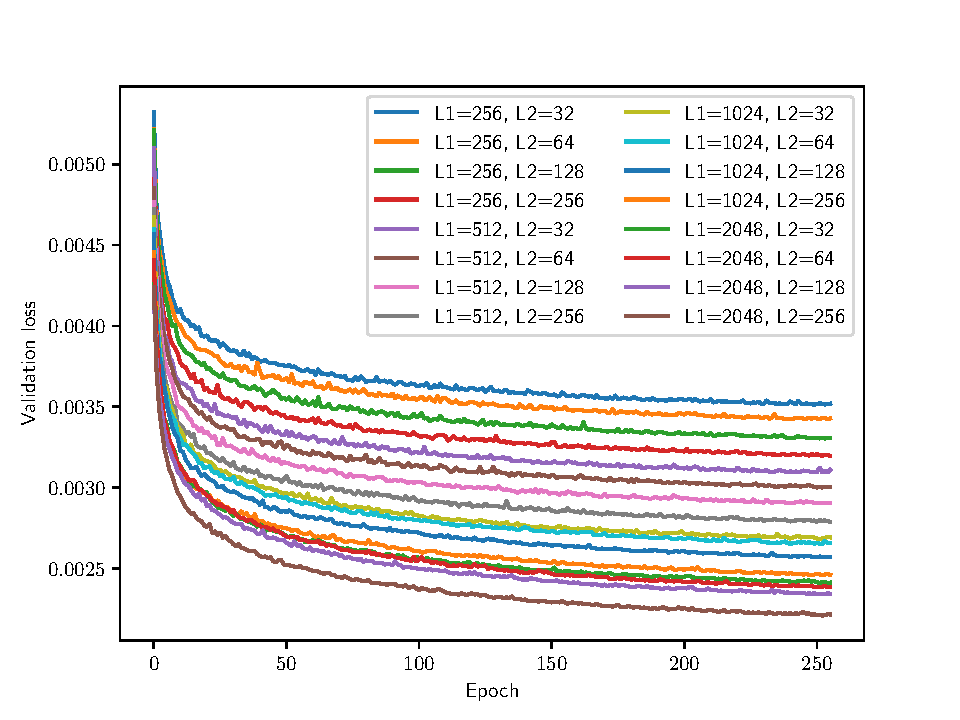
\includegraphics[width=\textwidth]{./dynamic/output/baseline_val_loss.pdf}}
\caption{Network architecture sweep validation loss over epochs (baseline)}
\end{figure}

%%%%%%%%%%%%%%%%%%%%%%%%%%%%%%%%%%%%%%%%%%%%%%%%%%%%%%%%%%%%%%%%%%%
%%%%%%%%%%%%%%%%%%%%%%%%%%%%%%%%%%%%%%%%%%%%%%%%%%%%%%%%%%%%%%%%%%%
%%%%%%%%%%%%%%%%%%%%%%%%%%%%%%%%%%%%%%%%%%%%%%%%%%%%%%%%%%%%%%%%%%%
%%%%%%%%%%%%%%%%%%%%%%%%%%%%%%%%%%%%%%%%%%%%%%%%%%%%%%%%%%%%%%%%%%%
%%%%%%%%%%%%%%%%%%%%%%%%%%%%%%%%%%%%%%%%%%%%%%%%%%%%%%%%%%%%%%%%%%%
%%%%%%%%%%%%%%%%%%%%%%%%%%%%%%%%%%%%%%%%%%%%%%%%%%%%%%%%%%%%%%%%%%%
%%%%%%%%%%%%%%%%%%%%%%%%%%%%%%%%%%%%%%%%%%%%%%%%%%%%%%%%%%%%%%%%%%%

\newpage
\subsection{Axis encoding}
\label{appendix:axes}

\subsubsection{Examples}
\label{appendix:axis_samples}

\begin{figure}[H]
\centering
\subfloat[\centering $\white$ White]{{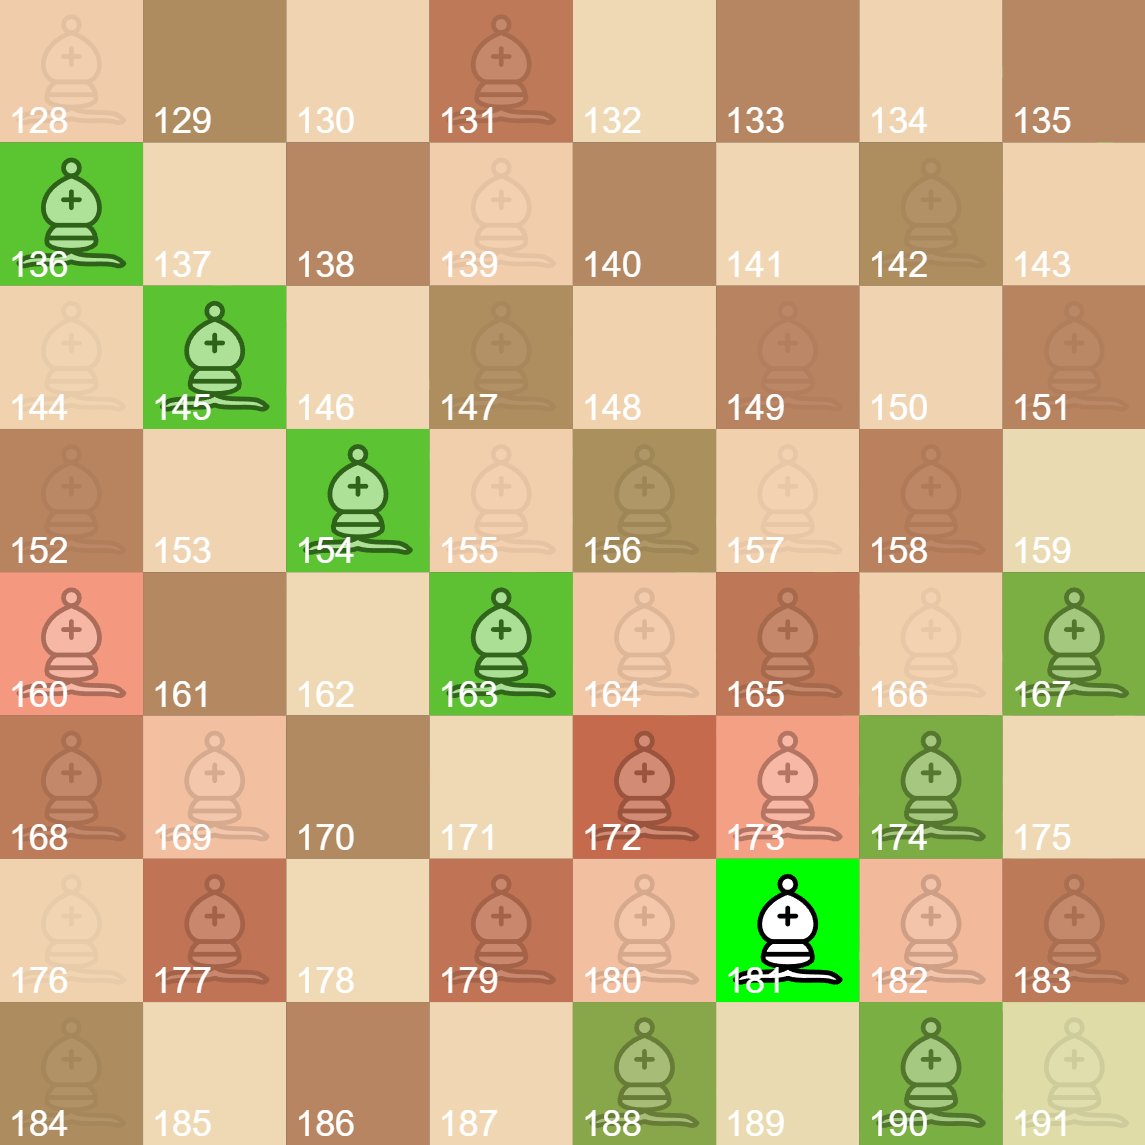
\includegraphics[width=4.65cm]{../assets/results/piece_weights/white_bishop_weights.png} }}
\qquad
\subfloat[\centering $\white$ White]{{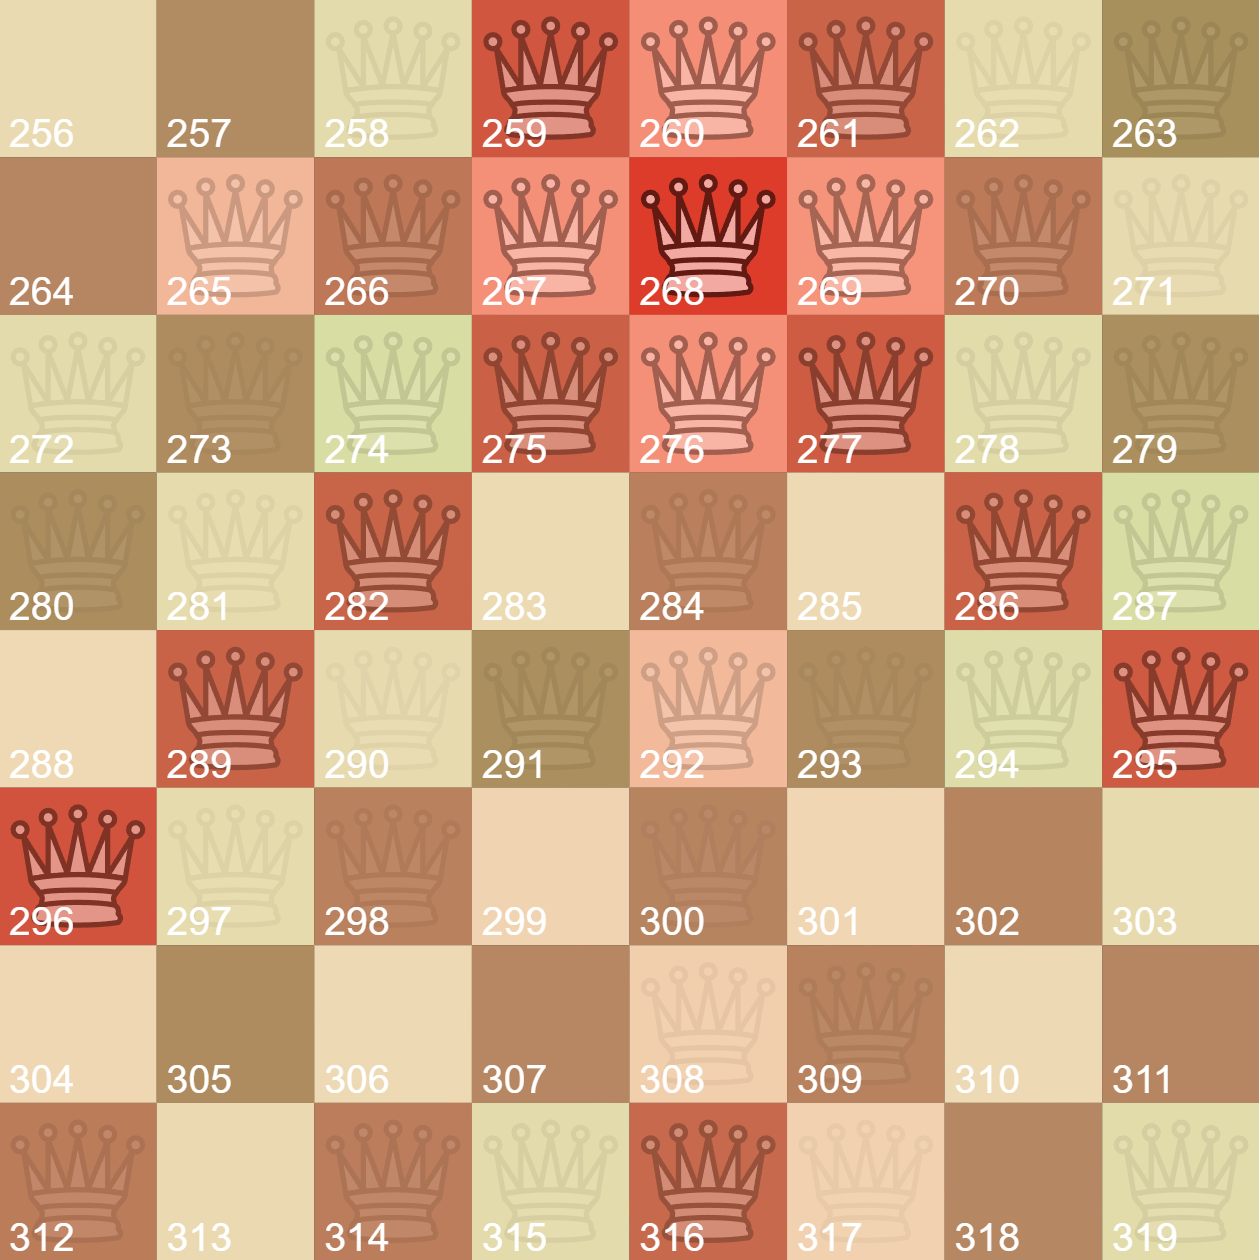
\includegraphics[width=4.65cm]{../assets/results/piece_weights/white_queen_weights.png} }}
\qquad
\subfloat[\centering $\white$ White]{{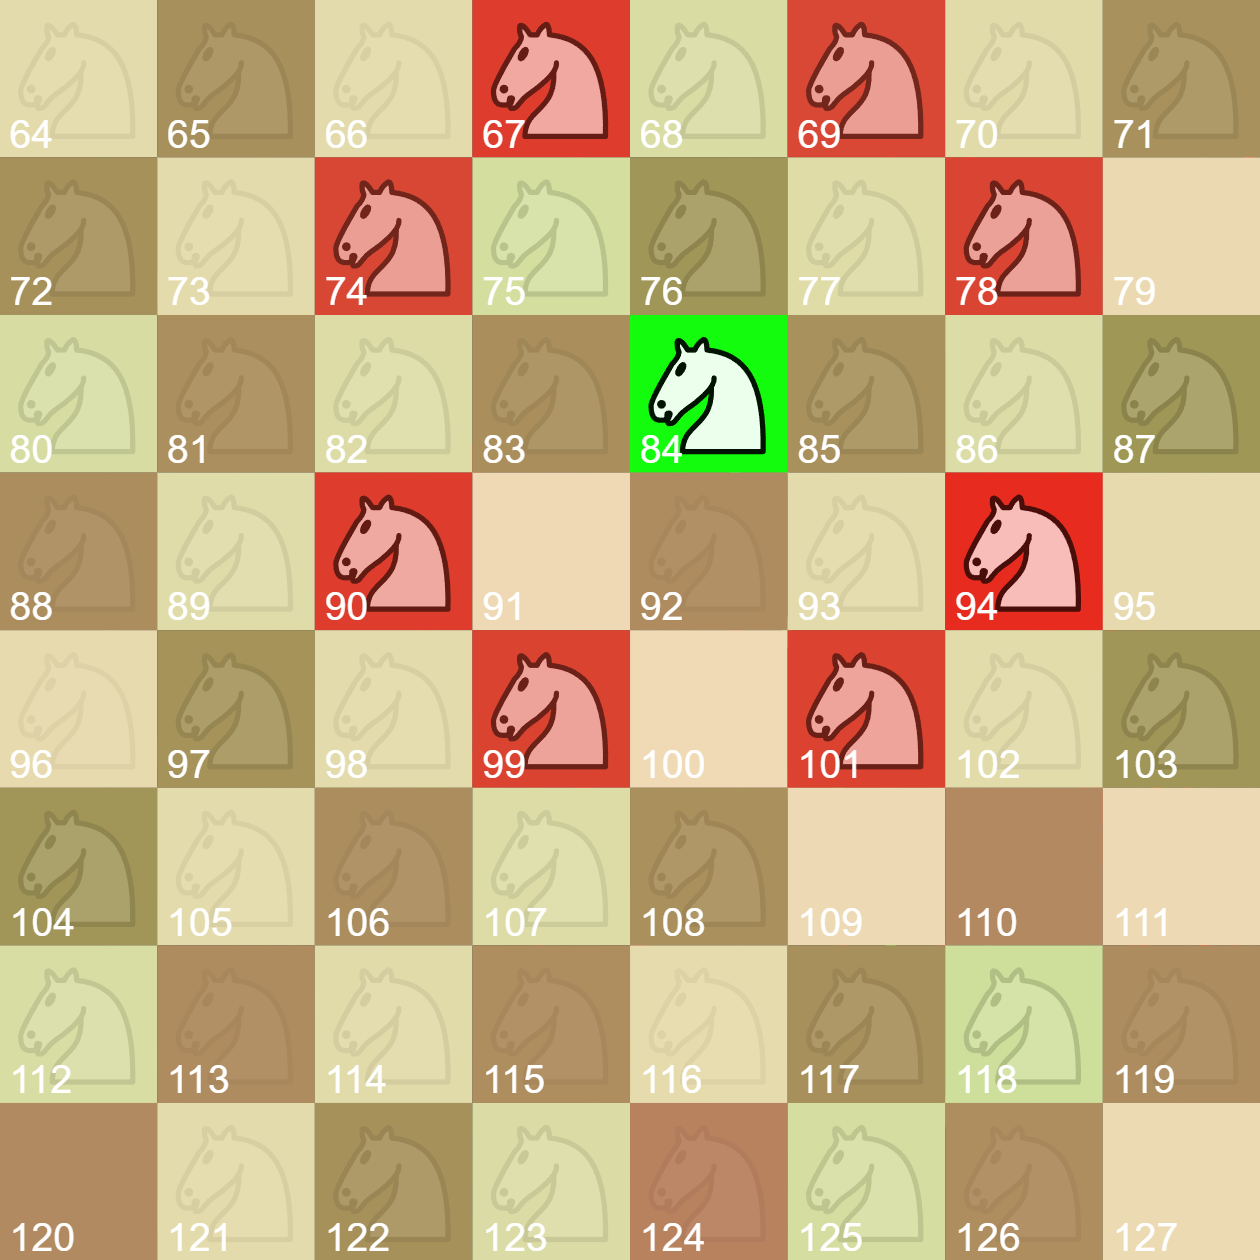
\includegraphics[width=4.65cm]{../assets/results/piece_weights/white_knight_weights.png} }} \\

\subfloat[\centering $\black$ Black]{{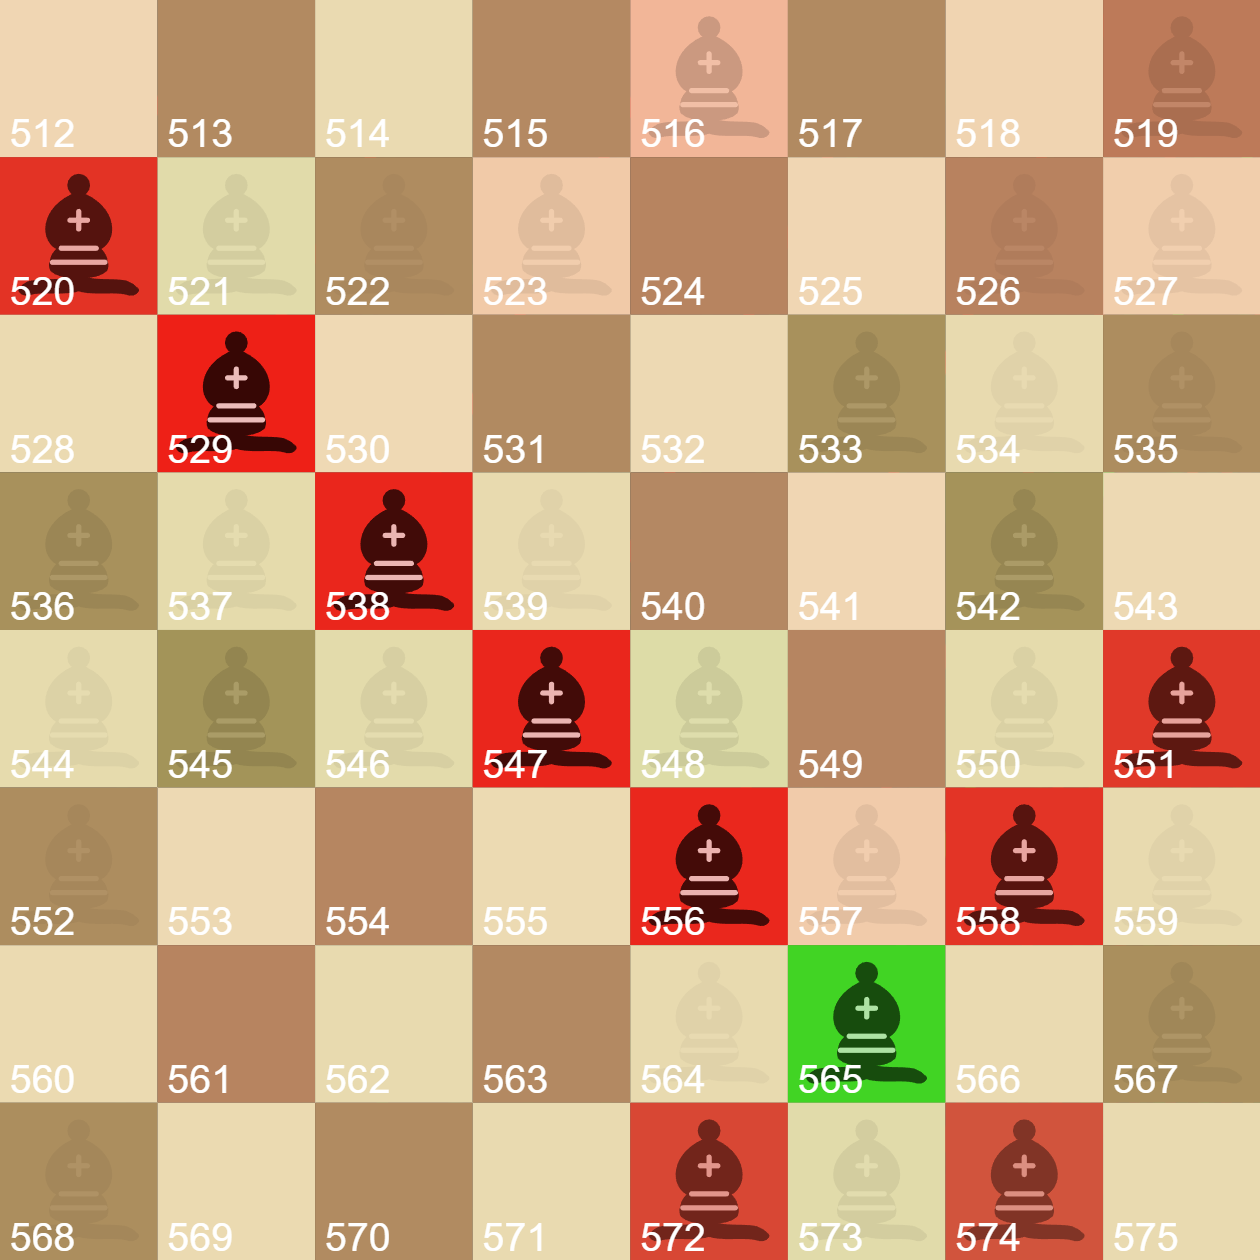
\includegraphics[width=4.65cm]{../assets/results/piece_weights/black_bishop_weights.png} }}
\qquad
\subfloat[\centering $\black$ Black]{{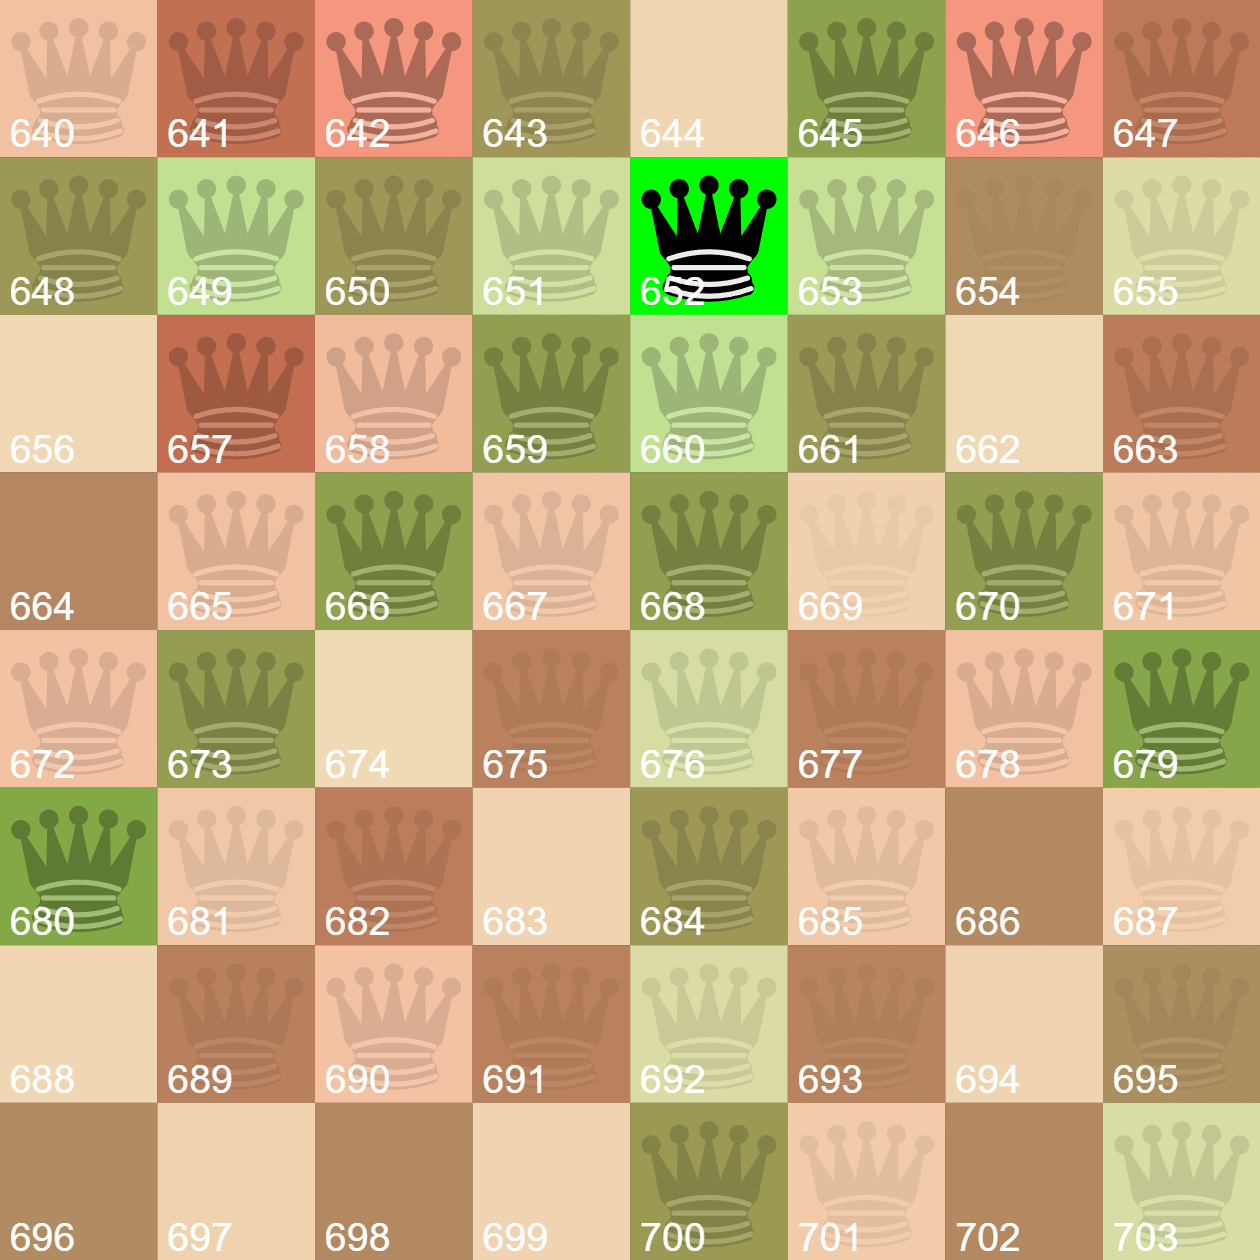
\includegraphics[width=4.65cm]{../assets/results/piece_weights/black_queen_weights.png} }}
\qquad
\subfloat[\centering $\black$ Black]{{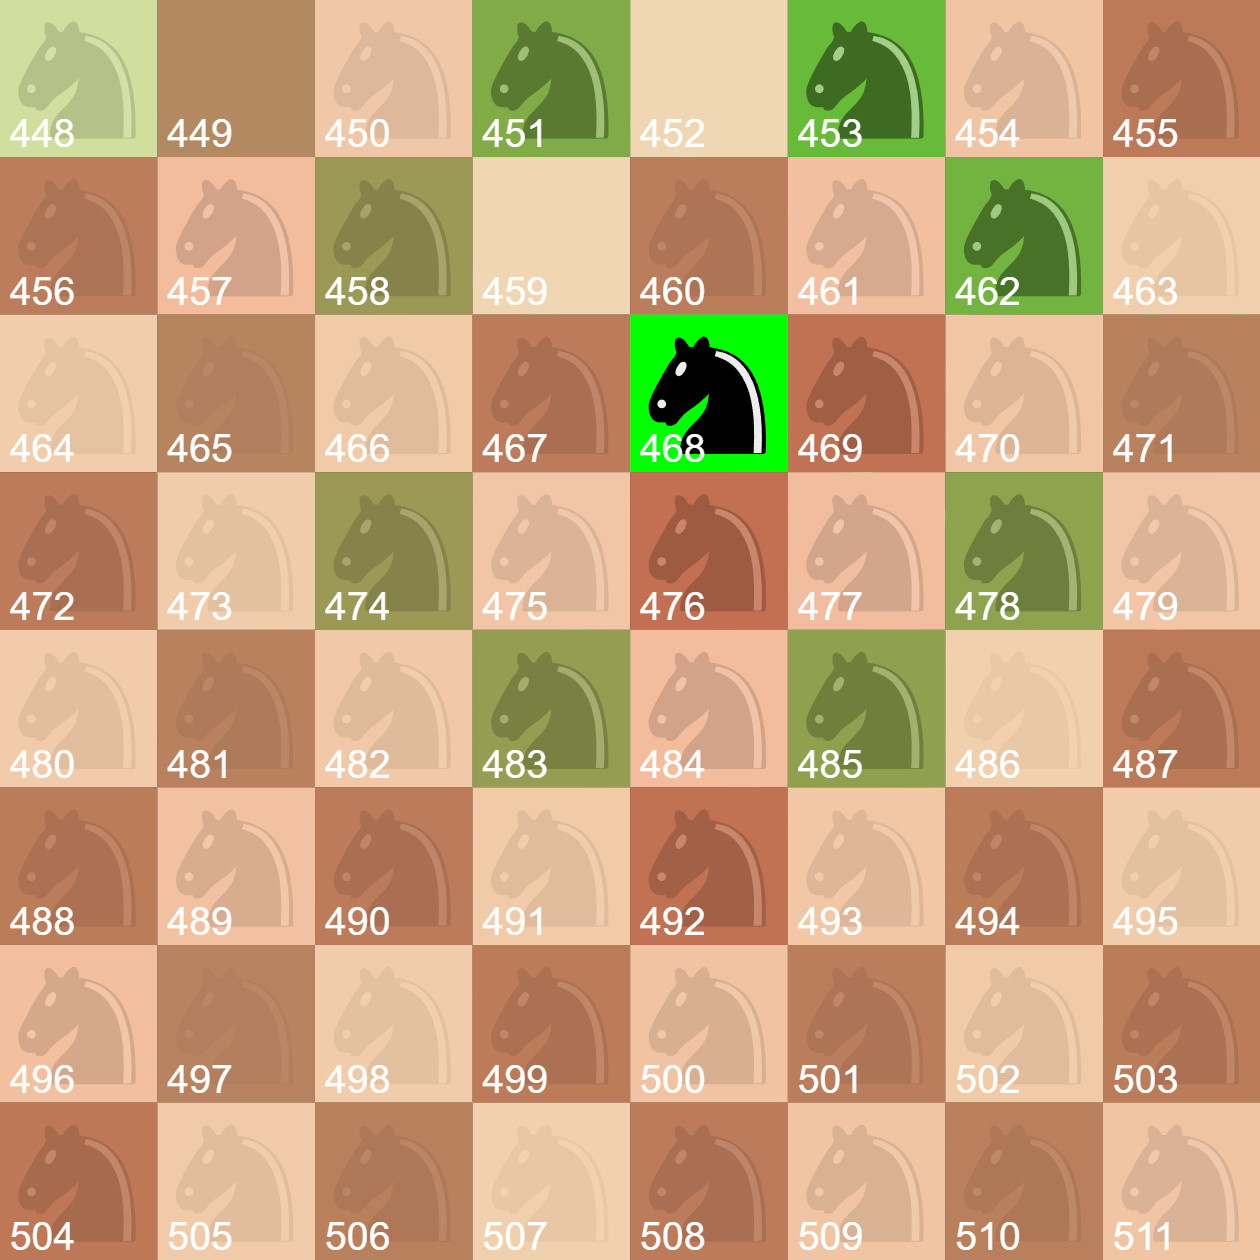
\includegraphics[width=4.65cm]{../assets/results/piece_weights/black_knight_weights.png} }} \\

\caption{Weights of different neurons in the L1 layer, which are connected to features in \featureset{All} with different roles. The intensity represents the weight value, and the color represents the sign. The number is the feature index, specifically \featureset{VH} instead of \featureset{HV} (both are \featureset{All}), because it was prior to the first experiment. Refer to section \ref{sec:axis_encoding}.}
\end{figure}


\subsubsection{Preliminar runs}

    \begin{table}[H]
\caption{Axis feature sets preliminar runs}
\centering
\begin{adjustbox}{center}
\begin{tabular}{@{} cccc|cc @{}}
\toprule
\bf \multirow{2}{*}{Feature set} & \bf \multirow{2}{*}{Run} & \bf Val. loss & \bf Runtime & \bf Rating @ 192 & \bf Rating @ 256 \\
 &  & \textit{min} & \textit{hh:mm:ss} & \textit{TC=100ms/m} & \textit{TC=100ms/m} \\
\midrule
    \multirow{4}{*}{\featureset{D1} + \featureset{D2}} & 1 & \bf0.006707 & 1:44:25 & 2.1 $\pm$ 4.3 & \bf13.5 $\pm$ 4.6\\
 & 2 & 0.006716 & 1:45:46 & -3.9 $\pm$ 5.1 & -0.5 $\pm$ 5.0\\
 & 3 & 0.006729 & 1:47:58 & -4.7 $\pm$ 4.8 & -1.6 $\pm$ 5.3\\
 & 4 & 0.006721 & 1:51:24 & -0.9 $\pm$ 5.3 & -4.0 $\pm$ 5.0\\
\midrule
\multirow{4}{*}{\featureset{H} + \featureset{V}} & 1 & \bf0.005810 & 1:42:35 & -8.6 $\pm$ 5.2 & \bf9.5 $\pm$ 5.5\\
 & 2 & 0.005827 & 1:42:29 & -2.6 $\pm$ 5.4 & -6.5 $\pm$ 5.1\\
 & 3 & 0.005816 & 1:42:59 & 4.8 $\pm$ 4.8 & 2.4 $\pm$ 5.4\\
 & 4 & 0.005825 & 1:43:13 & -6.3 $\pm$ 4.9 & 7.4 $\pm$ 5.2\\
\midrule
\multirow{4}{*}{\featureset{H} + \featureset{V} + \featureset{D1} + \featureset{D2}} & 1 & \bf0.003885 & 2:26:05 & -14.3 $\pm$ 4.9 & -18.1 $\pm$ 4.3\\
 & 2 & 0.003907 & 2:27:30 & 7.2 $\pm$ 5.0 & \bf15.4 $\pm$ 4.7\\
 & 3 & 0.003905 & 2:27:35 & 0.1 $\pm$ 5.3 & 5.2 $\pm$ 4.4\\
 & 4 & 0.003906 & 2:45:19 & 5.7 $\pm$ 5.0 & -1.2 $\pm$ 4.5\\
\midrule
\multirow{4}{*}{\featureset{All}} & 1 & \bf0.003121 & 1:30:34 & -2.9 $\pm$ 4.7 & 4.6 $\pm$ 4.4\\
 & 2 & 0.003129 & 1:30:13 & -4.2 $\pm$ 5.0 & 10.1 $\pm$ 5.4\\
 & 3 & 0.003134 & 1:30:14 & -10.0 $\pm$ 5.2 & \bf10.4 $\pm$ 5.1\\
 & 4 & 0.003147 & 1:30:18 & -9.6 $\pm$ 5.0 & 1.6 $\pm$ 4.8\\
\midrule
\multirow{4}{*}{\featureset{All} + \featureset{D1} + \featureset{D2}} & 1 & 0.003093 & 2:06:54 & -5.0 $\pm$ 4.4 & 1.7 $\pm$ 4.5\\
 & 2 & \bf0.003087 & 2:12:30 & 8.6 $\pm$ 4.3 & \bf12.0 $\pm$ 4.7\\
 & 3 & \bf0.003087 & 2:26:29 & -3.1 $\pm$ 4.9 & 7.9 $\pm$ 3.9\\
 & 4 & 0.003095 & 2:38:25 & -6.1 $\pm$ 4.5 & -16.0 $\pm$ 4.4\\
\midrule
\multirow{4}{*}{\featureset{All} + \featureset{H} + \featureset{V}} & 1 & 0.003086 & 2:05:02 & 1.0 $\pm$ 4.8 & 9.0 $\pm$ 6.0\\
 & 2 & 0.003082 & 2:06:16 & \bf12.9 $\pm$ 4.8 & 7.1 $\pm$ 5.5\\
 & 3 & \bf0.003079 & 2:04:53 & -14.6 $\pm$ 5.1 & 2.3 $\pm$ 5.5\\
 & 4 & 0.003085 & 2:07:18 & -10.1 $\pm$ 4.9 & -7.6 $\pm$ 4.4\\
\midrule
\multirow{4}{*}{\featureset{All} + \featureset{H} + \featureset{V} + \featureset{D1} + \featureset{D2}} & 1 & 0.003071 & 2:49:23 & -18.7 $\pm$ 4.9 & 4.3 $\pm$ 4.6\\
 & 2 & 0.003052 & 2:42:18 & -6.6 $\pm$ 4.6 & -0.6 $\pm$ 4.8\\
 & 3 & 0.003067 & 2:44:26 & 6.5 $\pm$ 4.8 & \bf9.5 $\pm$ 4.6\\
 & 4 & \bf0.003050 & 2:44:34 & -2.9 $\pm$ 5.4 & 8.5 $\pm$ 4.6\\
\toprule
\multicolumn{6}{c}{\makecell{\textbf{Batch size}: 16384, \textbf{LR}: 5e-04, \textbf{Gamma}: 0.99, \textbf{L1}: 512, \textbf{L2}: 32}} \\
\end{tabular}
\end{adjustbox}
\end{table}


\subsubsection{Final results}

    \begin{table}[H]
\caption{Axes feature sets final results}
\centering
\begin{adjustbox}{center}
\begin{tabular}{@{} cccc|cc @{}}
\toprule
\bf \multirow{2}{*}{Feature set} & \bf \multirow{2}{*}{Run} & \bf Val. loss & \bf Runtime & \bf Rating @ 192 & \bf Rating @ 256 \\
 &  & \textit{min} & \textit{hh:mm:ss} & \textit{TC=100ms/m} & \textit{TC=100ms/m} \\
\midrule
    \midrule
\multicolumn{6}{c}{\makecell{None}} \\
\end{tabular}
\end{adjustbox}
\end{table}




%%%%%%%%%%%%%%%%%%%%%%%%%%%%%%%%%%%%%%%%%%%%%%%%%%%%%%%%%%%%%%%%%%%
%%%%%%%%%%%%%%%%%%%%%%%%%%%%%%%%%%%%%%%%%%%%%%%%%%%%%%%%%%%%%%%%%%%
%%%%%%%%%%%%%%%%%%%%%%%%%%%%%%%%%%%%%%%%%%%%%%%%%%%%%%%%%%%%%%%%%%%
%%%%%%%%%%%%%%%%%%%%%%%%%%%%%%%%%%%%%%%%%%%%%%%%%%%%%%%%%%%%%%%%%%%
%%%%%%%%%%%%%%%%%%%%%%%%%%%%%%%%%%%%%%%%%%%%%%%%%%%%%%%%%%%%%%%%%%%
%%%%%%%%%%%%%%%%%%%%%%%%%%%%%%%%%%%%%%%%%%%%%%%%%%%%%%%%%%%%%%%%%%%
%%%%%%%%%%%%%%%%%%%%%%%%%%%%%%%%%%%%%%%%%%%%%%%%%%%%%%%%%%%%%%%%%%%

\newpage
\subsection{Pairwise runs}
\label{appendix:pairwise}

\subsubsection{Preliminar runs}

    \begin{table}[H]
\caption{Pairwise feature sets preliminar runs}
\centering
\begin{adjustbox}{center}
\begin{tabular}{@{} cccc|cc @{}}
\toprule
\bf \multirow{2}{*}{Feature set} & \bf \multirow{2}{*}{Run} & \bf Val. loss & \bf Runtime & \bf Rating @ 192 & \bf Rating @ 256 \\
 &  & \textit{min} & \textit{hh:mm:ss} & \textit{TC=100ms/m} & \textit{TC=100ms/m} \\
\midrule
    \multirow{4}{*}{\featureset{All} + \featureset{PH}} & 1 & 0.002954 & 1:56:52 & -2.9 $\pm$ 4.5 & 3.8 $\pm$ 4.0\\
 & 2 & 0.002969 & 1:56:24 & 1.7 $\pm$ 4.7 & 3.3 $\pm$ 4.7\\
 & 3 & 0.002953 & 1:56:12 & -8.7 $\pm$ 4.9 & -1.4 $\pm$ 4.4\\
 & 4 & \bf0.002946 & 1:56:33 & -8.8 $\pm$ 4.7 & \bf13.0 $\pm$ 4.7\\
\midrule
\multirow{4}{*}{\featureset{All} + \featureset{PH} + \featureset{PH}} & 1 & \bf0.002860 & 3:08:28 & -17.9 $\pm$ 5.4 & -5.4 $\pm$ 4.9\\
 & 2 & 0.002865 & 4:10:56 & 1.7 $\pm$ 5.6 & 7.8 $\pm$ 5.5\\
 & 3 & 0.002873 & 3:41:16 & -5.3 $\pm$ 5.0 & 6.2 $\pm$ 5.1\\
 & 4 & 0.002868 & 3:41:38 & 0.8 $\pm$ 5.3 & \bf12.0 $\pm$ 4.9\\
\midrule
\multirow{4}{*}{\featureset{All} + \featureset{PH}} & 1 & \bf0.003022 & 1:57:13 & 2.4 $\pm$ 4.4 & 6.7 $\pm$ 4.6\\
 & 2 & 0.003023 & 2:31:41 & -5.5 $\pm$ 4.6 & 1.8 $\pm$ 4.4\\
 & 3 & 0.003053 & 2:42:28 & -21.7 $\pm$ 4.7 & 0.8 $\pm$ 4.2\\
 & 4 & 0.003033 & 2:44:46 & 7.5 $\pm$ 4.5 & \bf8.0 $\pm$ 4.5\\
\toprule
\multicolumn{6}{c}{\makecell{\textbf{Batch size}: 16384, \textbf{LR}: 5e-04, \textbf{Gamma}: 0.99, \textbf{L1}: 512, \textbf{L2}: 32}} \\
\end{tabular}
\end{adjustbox}
\end{table}


\subsubsection{Final results}

    \begin{table}[H]
\caption{Pairwise feature sets final results}
\centering
\begin{adjustbox}{center}
\begin{tabular}{@{} cccccc @{}}
\toprule
\bf \multirow{2}{*}{Feature set} & \bf \multirow{2}{*}{Run} & \bf \multirow{2}{*}{Epoch} & \bf Val. loss  & \bf Rating & \bf TBD \\
 &  &  & \textit{min}  & \textit{TC=100ms/m} &  \\
\midrule
    \featureset{All} + \featureset{PH} & 4 & 256 & 0.002946 & \bf-8.4 $\pm$ 5.0\\
\featureset{All} + \featureset{PH} + \featureset{PV} & 4 & 256 & \bf0.002868 & -37.6 $\pm$ 4.9\\
\featureset{All} + \featureset{PV} & 4 & 256 & 0.003033 & -38.2 $\pm$ 4.8\\
\toprule
\multicolumn{6}{c}{\makecell{\textbf{Batch size}: 16384, \textbf{LR}: 5e-04, \textbf{Gamma}: 0.99, \textbf{L1}: 512, \textbf{L2}: 32}} \\
\end{tabular}
\end{adjustbox}
\end{table}



%%%%%%%%%%%%%%%%%%%%%%%%%%%%%%%%%%%%%%%%%%%%%%%%%%%%%%%%%%%%%%%%%%%
%%%%%%%%%%%%%%%%%%%%%%%%%%%%%%%%%%%%%%%%%%%%%%%%%%%%%%%%%%%%%%%%%%%
%%%%%%%%%%%%%%%%%%%%%%%%%%%%%%%%%%%%%%%%%%%%%%%%%%%%%%%%%%%%%%%%%%%
%%%%%%%%%%%%%%%%%%%%%%%%%%%%%%%%%%%%%%%%%%%%%%%%%%%%%%%%%%%%%%%%%%%
%%%%%%%%%%%%%%%%%%%%%%%%%%%%%%%%%%%%%%%%%%%%%%%%%%%%%%%%%%%%%%%%%%%
%%%%%%%%%%%%%%%%%%%%%%%%%%%%%%%%%%%%%%%%%%%%%%%%%%%%%%%%%%%%%%%%%%%
%%%%%%%%%%%%%%%%%%%%%%%%%%%%%%%%%%%%%%%%%%%%%%%%%%%%%%%%%%%%%%%%%%%

\newpage
\subsection{Mobility runs}
\label{appendix:mobility}

\subsubsection{Preliminar runs}
%
    \begin{table}[H]
\caption{Mobility feature sets preliminar runs}
\centering
\begin{adjustbox}{center}
\begin{tabular}{@{} cccc|cc @{}}
\toprule
\bf \multirow{2}{*}{Feature set} & \bf \multirow{2}{*}{Run} & \bf Val. loss & \bf Runtime & \bf Rating @ 192 & \bf Rating @ 256 \\
 &  & \textit{min} & \textit{hh:mm:ss} & \textit{TC=100ms/m} & \textit{TC=100ms/m} \\
\midrule
    \multirow{4}{*}{\featureset{All} + \featureset{MB}} & 1 & \bf0.002809 & 2:46:15 & 0.1 $\pm$ 5.7 & -7.5 $\pm$ 5.9\\
 & 2 & 0.002824 & 2:51:49 & -6.1 $\pm$ 6.1 & \bf12.1 $\pm$ 6.5\\
 & 3 & 0.002812 & 2:49:58 & -2.4 $\pm$ 5.2 & 11.4 $\pm$ 5.2\\
 & 4 & 0.002828 & 2:53:24 & -7.5 $\pm$ 6.0 & 0.0 $\pm$ 5.7\\
\midrule
\multirow{4}{*}{\featureset{All} + \featureset{MC}} & 1 & 0.003045 & 2:23:00 & 15.5 $\pm$ 5.2 & -30.5 $\pm$ 5.3\\
 & 2 & 0.003060 & 2:22:55 & -41.5 $\pm$ 5.5 & 2.6 $\pm$ 5.3\\
 & 3 & 0.003040 & 2:38:55 & 0.7 $\pm$ 5.4 & 12.6 $\pm$ 4.3\\
 & 4 & \bf0.003032 & 2:21:59 & 19.0 $\pm$ 5.6 & \bf21.5 $\pm$ 4.9\\
\toprule
\multicolumn{6}{c}{\makecell{\textbf{Batch size}: 16384, \textbf{LR}: 5e-04, \textbf{Gamma}: 0.99, \textbf{L1}: 512, \textbf{L2}: 32\\Each tournament rating is relative to its average (rating=0)}} \\
\end{tabular}
\end{adjustbox}
\end{table}


\subsubsection{Final results}
%
    \begin{table}[H]
\caption{Mobility feature sets final results}
\centering
\begin{adjustbox}{center}
\begin{tabular}{@{} ccccc @{}}
\toprule
\bf \multirow{2}{*}{Feature set} & \bf \multirow{2}{*}{Run} & \bf \multirow{2}{*}{Epoch} & \bf Val. loss  & \bf Rating \\
 &  &  & \textit{min}  & \textit{TC=100ms/m} \\
\midrule
    \featureset{All} + \featureset{MB} & 2 & 256 & \bf0.002824 & \bf-260.9 $\pm$ 5.4\\
\featureset{All} + \featureset{MC} & 4 & 256 & 0.003032 & -280.9 $\pm$ 5.6\\
\toprule
\multicolumn{5}{c}{\makecell{\textbf{Batch size}: 16384, \textbf{LR}: 5e-04, \textbf{Gamma}: 0.99, \textbf{L1}: 512, \textbf{L2}: 32\\Tournament rating is relative to \featureset{All} (rating=0)}} \\
\end{tabular}
\end{adjustbox}
\end{table}


%%%%%%%%%%%%%%%%%%%%%%%%%%%%%%%%%%%%%%%%%%%%%%%%%%%%%%%%%%%%%%%%%%%
%%%%%%%%%%%%%%%%%%%%%%%%%%%%%%%%%%%%%%%%%%%%%%%%%%%%%%%%%%%%%%%%%%%
%%%%%%%%%%%%%%%%%%%%%%%%%%%%%%%%%%%%%%%%%%%%%%%%%%%%%%%%%%%%%%%%%%%
%%%%%%%%%%%%%%%%%%%%%%%%%%%%%%%%%%%%%%%%%%%%%%%%%%%%%%%%%%%%%%%%%%%
%%%%%%%%%%%%%%%%%%%%%%%%%%%%%%%%%%%%%%%%%%%%%%%%%%%%%%%%%%%%%%%%%%%
%%%%%%%%%%%%%%%%%%%%%%%%%%%%%%%%%%%%%%%%%%%%%%%%%%%%%%%%%%%%%%%%%%%
%%%%%%%%%%%%%%%%%%%%%%%%%%%%%%%%%%%%%%%%%%%%%%%%%%%%%%%%%%%%%%%%%%%

\newpage
\subsection{\texttt{emitPlainEntry} code}
\label{appendix:emitPlainEntry}

\lstset{
  %backgroundcolor=\color{gray!10},  
  basicstyle=\ttfamily,
  columns=fullflexible,
  breakatwhitespace=false,      
  breaklines=true,                
  captionpos=b,                    
  commentstyle=\color{green}, 
  extendedchars=true,              
  frame=single,                   
  keepspaces=true,             
  keywordstyle=\color{blue},      
  language=c++,                 
  numbers=none,                
  numbersep=5pt,                   
  numberstyle=\tiny\color{blue},
  rulecolor=\color{white},        
  showspaces=false,               
  showtabs=false,                 
  stepnumber=5,                  
  stringstyle=\color{red!60!blue},
  tabsize=3,                      
  title=\lstname                
}
\begin{lstlisting}
void emitPlainEntry(std::string& buffer, const TrainingDataEntry& plain)
{
    buffer += plain.pos.fen();
    buffer += ',';
    buffer += std::to_string(plain.score);
    buffer += ',';
    buffer += chess::uci::moveToUci(plain.pos, plain.move);
    buffer += '\n';
}
\end{lstlisting}



\end{document}


% https://ctan.dcc.uchile.cl/info/symbols/comprehensive/symbols-a4.pdf
